\documentclass[12pt,twoside,a4paper]{report}

\usepackage[latin1]{inputenc}
\usepackage[english]{babel}
\usepackage{enumerate}
\usepackage{amsmath}
\usepackage{amssymb}
\usepackage{amsthm}
\usepackage{latexsym}
\usepackage{makeidx}
\usepackage[dvips]{graphicx}
%\usepackage{showidx}
\usepackage[retainorgcmds]{IEEEtrantools}

\makeindex

% --------------------------------------------------------------------- Symbols
\renewcommand{\phi}{\varphi}

% ------------------------------------------------------------------------ Sets
\newcommand{\N}{\mathbb{N}}
\newcommand{\R}{\mathbb{R}}
\newcommand{\Rplus}{\R^{+}}
\newcommand{\C}{\mathbb{C}}
\newcommand{\Z}{\mathbb{Z}}
\newcommand{\RS}{\hat{\C}}
\newcommand{\UnitCirc}{S^{1}}

\newcommand{\Words}[1]{{#1}^{\star}}

\newcommand{\GL}[1]{\operatorname{GL}_2(#1)}
\newcommand{\PGL}[1]{\operatorname{PGL}_2(#1)}
\newcommand{\SL}[1]{\operatorname{SL}_2(#1)}
\newcommand{\PSL}[1]{\operatorname{PSL}_2(#1)}
\newcommand{\Mat}[3]{{#1}^{#2 \times #3}}

\newcommand{\ModGrp}{\overline{\Gamma}}
\newcommand{\hModGrp}{\Gamma}

\newcommand{\setdef}[2]{\{#1 \mid #2\}}

% ---------------------------------------------------------------------- Macros
\newcommand{\todo}[2]{\bigskip\noindent\framebox[\textwidth]{\emph{TODO #1:} #2}\bigskip}
\newcommand{\ie}{i.e.\ }
\newcommand{\Wlog}{W.l.o.g.\ }
\newcommand{\txtiff}{if and only if\ }

% ------------------------------------------------------------------- Functions
\newcommand{\half}[1]{\frac{#1}{2}}
\newcommand{\reci}[1]{\frac{1}{#1}}

\newcommand{\cfr}[2]{
\begin{array}{c}\multicolumn{1}{c|}{#1}\\
\hline\multicolumn{1}{|c}{#2}\end{array}}

\newcommand{\inv}[1]{{#1}^{-1}}

\newcommand{\moebius}[5]{\frac{#1 #5 + #2}{#3 #5 + #4}}
\newcommand{\mat}[4]{\begin{pmatrix}#1 & #2 \\ #3 & #4\end{pmatrix}}
\newcommand{\rvec}[2]{\begin{pmatrix}#1 & #2\end{pmatrix}}
\newcommand{\cvec}[2]{\begin{pmatrix}#1 \\ #2\end{pmatrix}}
\newcommand{\htransp}[1]{#1^{\textrm{H}}}
\newcommand{\id}[1]{\operatorname{id}_{#1}}

\newcommand{\abs}[1]{|#1|}
\newcommand{\conj}[1]{\overline{#1}}
\renewcommand{\Re}[1]{\operatorname{Re}\left(#1\right)}
\renewcommand{\Im}[1]{\operatorname{Im}\left(#1\right)}

\newcommand{\epo}[1]{e^{#1}}
\newcommand{\ii}{i}

% ---------------------------------------------------------------- Environments

\newtheorem{theorem}{Theorem}[chapter]
\newtheorem{corollary}[theorem]{Corollary}
\newtheorem{lemma}[theorem]{Lemma}

\theoremstyle{definition}
\newtheorem{definition}[theorem]{Definition}
\newtheorem{example}[theorem]{Example}

\theoremstyle{remark}
\newtheorem*{remark}{Remark}


\title{Computer Algebra and Analysis:\\Complex Variables Visualized}
\author{Thomas Ponweiser}
\date{\today}

\begin{document}

\maketitle

\pagestyle{headings}

\tableofcontents

% ------------------------------------------------------- CHAPTER: INTRODUCTION
\chapter{Introduction}

% -------------------------------------------- Section: Algebraic constructions
\section{Groups and basic algebraic constructions}

In this section, we will recapitulate some basic algebraic concepts, most important the notions of \emph{free groups} and \emph{free products}, and the construction of a group in terms of \emph{generators} and \emph{relations}. Additionally, we give the definitions of the \emph{(projective) general} and \emph{special linear groups}. Lastly, \emph{group actions} on sets will be introduced. A reader familiar to this concepts may readily skip this section. Moreover, we will give no rigorous proofs here, as they may be found in many algebra books, as for example in \Hungerford.

\subsection{Groups and homomorphisms}

\index{Binary!operation}
If $G$ is a nonempty set, a \emph{binary operation} on $G$ is a function $G \times G \to G$. Commonly used notations for the image of $(a,b) \in G \times G$ under a binary operation are $a \cdot b$ or $ab$ (product notation), $a + b$ (additive notation), $a \circ b$, $a \ast b$, etc. In this chapter and also later on we will use the \emph{product notation}, $(a,b) \mapsto a \cdot b =  ab$, most frequently and we refer to $ab$ as the \emph{product} of $a$ and $b$.

\begin{definition}[Groups and monoids]
\label{dfn_GroupMonoid}
\index{Group}
\index{Monoid}
Let $G$ be a nonempty set together with a binary operation on $G$. If the binary operation satisfies the following three axioms,
\index{Associativity}
\begin{enumerate}[(i)]
\item \label{itm_Associativity} \emph{Associativity:} $\forall a,b,c \in G: a(bc) = (ab)c$,
\item \label{itm_IdentityExists} \emph{Existence of an identity element:} $\exists e \in G\ \forall a \in G: ea = ae = a$,
\item \emph{Existence of inverse elements:} $\forall a \in G\ \exists \inv{a} \in G: a \inv{a} = \inv{a} a = e$,
\end{enumerate}
then $G$ is called a \emph{group}. If the axioms (\ref{itm_Associativity}) and (\ref{itm_IdentityExists}) are satisfied, then $G$ is called a \emph{monoid}. Of course every group is in particular monoid. The notation $\langle G,\cdot,e \rangle$ will be used for making the identity element and the involved binary operation explicit.
\end{definition}

It is convenient to introduce the following notations operating on subsets of a group $G$. For $g \in G$ and $A,B \subseteq G$ we define
\begin{eqnarray*}
\inv{A} &:=& \setdef{\inv{a}}{a \in A} \subseteq G, \\
AB &:=& \setdef{a b}{a \in A, b \in B} \subseteq G,\\
gA &:=& \{g\}A = \setdef{g a}{a \in A} \subseteq G,\\
Ag &:=& A\{g\} = \setdef{a g}{a \in A} \subseteq G.
\end{eqnarray*}

\begin{definition}[Subgroups]
\label{dfn_Subgroup}
\index{Subgroup}
Let $\langle G,\cdot,e \rangle$ be a group. A nonempty subset $H \subseteq G$ which is closed under the binary operation $\cdot$ and inversion, \ie $H\inv{H} = H$, is called a \emph{subgroup} of $G$, in symbols $H \le G$. In particular, $\langle H,\cdot,e \rangle$ is itself a group. If $H \le G$ and $H \ne G$, $H$ is called a \emph{proper subgroup} of $G$, and we write $H \lneq G$. The subgroup $\{e\} \le G$ is called the \emph{trivial subgroup}.
\end{definition}

\index{Conjuagtion}
If $H$ is a subgroup of $G$, then for every $g \in G$ also $gH\inv{g}$ is a subgroup of $G$. For $h \in H$, $g \in G$, we call the operation $h \mapsto g h \inv{g}$ \emph{conjugation} of $h$ by $g$.

\begin{definition}[Normal subgroups]
\label{dfn_NormalSubgroup}
A subgroup $N$ of a group $G$ which is closed under conjugation by elements of $G$, \ie $g N \inv{g} = N$ for all $g \in G$, is called a \emph{normal subgroup} of $G$, in symbols $N \unlhd G$.
\end{definition}

If $N$ is a normal subgroup of $G$, then we have $gN = Ng$ for every $g \in G$, which is why we can define on the set
\begin{equation}
\label{eqn_FactorGroup}
G / N := \setdef{gN}{g \in G}
\end{equation}
a binary operation by $aNbN := abNN = abN$ for $a,b \in G$. It is easy to see that $G / N$ together with this operation forms a group.

\begin{definition}[Factor groups]
\label{dfn_FactorGroup}
Let $N$ be a normal subgroup of a group $G$. The set $G / N$ defined in (\ref{eqn_FactorGroup}) together with the binary operation $(aN,bN) \mapsto abN$ is called the \emph{factor group} (or \emph{quotient group}) of $G$ by $N$.
\end{definition}

\begin{definition}[Homomorphisms]
\label{dfn_Homomorphism}
\index{Homomorphism}
\index{Monomorphism}
\index{Epimorphism}
\index{Isomorphism}
\index{Endomorphism}
\index{Automorphism}
Let $G$ and $H$ be groups (or monoids). A function $f : G \to H$ is a \emph{homomorphism} from $G$ to $H$, if and only if
\begin{equation*}
f(ab) = f(a) f(b) \quad \text{for all } a,b \in G.
\end{equation*}
Depending on $f$ being injective and/or surjective, one distinguishes \emph{monomorphisms} ($f$ is injective), \emph{epimorphisms} ($f$ is surjective) and \emph{isomorphisms} ($f$ is bijective). We call the groups $G$ and $H$ \emph{isomorphic}, in symbols $G \cong H$, if and only if there exists and isomorphism $f : G \to H$. Finally, a homomorphism $f : G \to G$ of $G$ to itself is called \emph{endomorphism}. A bijective endomorphism is called \emph{automorphism}.
\end{definition}

\begin{definition}[Kernel]
\label{dfn_Kernel}
Let $G$ and $H$ be groups and denote the identity element of $H$ by $e_H$. For a homomorphism $f: G \to H$, the set
\begin{equation}
\ker f := \setdef{g \in G}{f(g) = e_H}
\end{equation}
is called the \emph{kernel} of f.
\end{definition}
\begin{lemma}
\label{lem_KernelAndImage}
Let $G$ and $H$ be groups and $f : G \to H$ be a homomorphism. The kernel of $f$ is a normal subgroup of $G$ and the image $f(G)$ is a subgroup of $H$:
\begin{equation*}
\ker f \unlhd G \quad \text{and} \quad f(G) \le H.
\end{equation*}
\end{lemma}
\begin{proof}
Denote the identity elements of $G$ and $H$ by $e_G$ and $e_H$ respectively. Because $f$ is a homomorphism, we have $f(e_G) = f(e_G e_G) = f(e_G) f(e_G)$. Multiplying this by $\inv{f(e_G)}$ yields $e_H = f(e_G)$. In other words $e_G \in \ker f$ and $\ker f$ is nonempty. To see that $\ker f \le G$, we need to show that for all $a, b \in \ker f$ also $a \inv{b} \in \ker f$ -- but this is easy:
\begin{equation*}
f(a \inv{b}) = f(a) f(\inv{b}) = f(a) \inv{f(b)} = e_H \inv{e_H} = e_H.
\end{equation*}
To see that $\ker f$ is a normal subgroup of $G$, let $a \in \ker f$, $g \in G$ and observe
\begin{equation*}
f(g a \inv{g}) = f(g) f(a) f(\inv{g}) = f(g) e_H \inv{f(g)} = e_H.
\end{equation*}
For this reason $g a \inv{g} \in \ker f$ and $\ker f$ is closed under conjugation by elements of $G$. For the second part of the prove, let $f(a), f(b) \in f(G)$ with $a,b \in G$. Clearly $f(a) \inv{f(b)} = f(a) f(\inv{b}) = f(a \inv{b}) \in f(G)$ and therefore $f(G) \le H$.
\end{proof}

\begin{theorem}[First isomorphism theorem]
\label{thm_FirstIsoThm}
Let $G$ and $H$ be groups and $f: G \to H$ be a homomorphism. Then the quotient group $G / \ker f$ is isomorphic to $f(G)$:
\begin{equation*}
G / \ker f \cong f(G).
\end{equation*}
\end{theorem}
\begin{proof}
Let us again denote the identity element of $H$ by $e_H$. Define $N := \ker f$ and a map $\phi : G/N \to f(G)$ by $aN \mapsto f(a)$. Now, for arbitrary $a,b \in G$ observe
\begin{equation*}
aN = bN \Leftrightarrow
a \inv{b} \in N \Leftrightarrow
e_H = f(a \inv{b}) = f(a) \inv{f(b)} \Leftrightarrow
f(a) = f(b).
\end{equation*}
This shows two things: First ($\Rightarrow$), $\phi$ is well defined and second ($\Leftarrow$), $\phi$ is injective. Clearly, $\phi$ is also surjective and by definition we have
\begin{equation*}
\phi(aN) \phi(bN) = f(a) f(b) = f(ab) = \phi(abN) \quad \text{for all } a,b \in G.
\end{equation*}
Therefore $\phi$ is indeed an isomorphism from $G/N$ to $f(G)$.
\end{proof}

\subsection{Free monoids}
\index{Free!monoid}
Let $\Syms$ be a set of formal symbols, for example $\Syms = \{a, b, c, \dots\}$. For $n \in \N$, $n \ge 0$, we denote by $\Syms^n$ the set of tuples of length $n$ over $\Syms$ and we will call these tuples \emph{words of length $n$ over the alphabet $\Syms$}. For simplicity, we will omit parentheses and commas when notating such a word, for example $(a,b,b,a) =: abba \in \Syms^4$ is a word of length 4. Note the special case for $n = 0$. By definition, $\Syms^0$ contains all words of length $0$. Obviously, there is only one such word, the so-called \emph{empty word}, which we denote by $\epsilon$. A second special case occurs for $\Syms = \emptyset$, where $\Syms^n = \emptyset$ for all $n > 0$ and $\Syms^0 = \{\epsilon\}$, because there are no words over the empty alphabet except the empty word. Next, we define 
\begin{equation}
\label{eqn_SigmaStarDef}
\Words{\Syms} := \bigcup_{n \ge 0} \Syms^n.
\end{equation}
as the set of all \emph{words over the alphabet $\Syms$}. It is now just natural to define a binary operation $\cdot$ on $\Words{\Syms}$ which is given by concatenation of words:
\begin{equation*}
w_1 \cdot w_2 := w_1 w_2, \quad w_1, w_2 \in \Words{\Syms}.
\end{equation*}
\index{Monoid}
Since $\Words{\Syms}$ together with the operation $\cdot$ satisfies the axioms of \emph{associativity},
\begin{equation*}
\forall w_1,w_2,w_3 \in \Words{\Syms}:\quad (w_1 \cdot w_2) \cdot w_3 = w_1 \cdot (w_2 \cdot w_3)
\end{equation*}
and \emph{existence of an identity element},
\begin{equation*}
\forall w \in \Words{\Syms}:\quad w \cdot  \epsilon = \epsilon \cdot w = w,
\end{equation*}
the algebraic structure $\langle \Words{\Syms}, \cdot, \epsilon \rangle$ forms a \emph{monoid}.

\begin{definition}[Free monoid]
\label{dfn_FreeMonoid}
Let $\Syms$ be an arbitrary set of symbols (called the alphabet), and $\Words{\Syms}$ be defined as in (\ref{eqn_SigmaStarDef}). Moreover, denote concatenation of words by $\cdot$ and let $\epsilon$ be the empty word. Then the algebraic structure $\langle \Words{\Syms}, \cdot, \epsilon \rangle$ is called the \emph{free monoid over the alphabet $\Syms$}.
\end{definition} 

\subsection{Free groups}
\index{Free!group}
\index{Formal!inverse}
In a similar fashion, we can construct also a group from any given formal alphabet $\Syms$. For this purpose we first choose a ``disjoint copy'' of $\Syms$ which we denote by $\inv{\Syms}$. To be precise, $\inv{\Syms}$ may be any arbitrary set satisfying $\Syms \cap \inv{\Syms} = \emptyset$ and having same cardinality as $\Syms$. In particular we could for example set $\inv{\Syms} := \Syms \times \{1\}$. Next, we choose a bijection $f : \Syms \to \inv{\Syms}$. We can extend this bijection between the sets $\Syms$ and $\inv{\Syms}$ to an involution $\overline{f}$ living on the union $\overline{\Syms} := \Syms \cup \inv{\Syms}$ by defining $\overline{f} := f \cup \inv{f}$ or more verbose:
\begin{equation*}
\overline{f}(a) := \begin{cases}
f(a)       & \text{if } a \in \Syms\\
\inv{f}(a) & \text{if } a \in \inv{\Syms}
\end{cases}
\end{equation*}
Now we introduce the notation $\overline{f}(a) =: \inv{a}$ for all $a \in \overline{\Syms}$ and call $\inv{a}$ the \emph{(formal) inverse} of the element $a$. 

\index{Reduced form}
\index{Group!word}
Having now defined a formal inverse for each of our symbols in the given alphabet, we can go on and consider the free monoid $\Words{\overline{\Syms}}$. If $\sigma_1, \sigma_2, \dots, \sigma_n$ are symbols of $\overline{\Syms}$, then we say the word $\sigma_1 \sigma_2 \dots \sigma_n$ is \emph{reduced}, if and only if no two subsequent symbols of the word are inverse to each other, that is
\begin{equation}
\label{eqn_GrpWordReducedForm}
 \sigma_j \ne \sigma_{j+1}^{-1} \quad \text{for all } 1 \le j < n.
\end{equation}
Clearly, every word $w \in \Words{\overline{\Syms}}$ can be brought into reduced form by successively ``canceling out'' adjacent inverse symbols until finally a word is obtained, which satisfies (\ref{eqn_GrpWordReducedForm}). We call the result of this procedure the \emph{reduced form of $w$}. Additionally, we define two words $w_1, w_2 \in \Words{\overline{\Syms}}$ to be \emph{equivalent}, if and only if they have the same reduced form and we write $w_1 \sim w_2$ in this case. If we denote the reduced form of $w$ by $\phi(w)$, we can write
\begin{equation*}
w_1 \sim w_2 \Leftrightarrow \phi(w_1) = \phi(w_2).
\end{equation*}
Moreover, we observe that if $w_1 \sim w_2$ and $v_1 \sim v_2$, then we also have $w_1 v_1 \sim w_2 v_2$ because $\phi(w_1) = \phi(w_2) =: w$ and $\phi(v_1) = \phi(v_2) =: v$ implies 
\begin{equation*}
\phi(w_1 v_1) = \phi(w v) = \phi(w_2 v_2).
\end{equation*}
Thus we see that the equivalence relation $\sim$ is compatible with the operation of word-concatenation. Therefore we can consider also the set of equivalence classes $\Words{\overline{\Syms}}/{\sim}$ as a monoid under the operation of word-concatenation. Obviously the set of reduced words is a system of representatives for $\Words{\overline{\Syms}}/{\sim}$ and we agree to denote an equivalence class $[w]_{\sim}$ simply by the reduced word $w$. $\Words{\overline{\Syms}}/{\sim}$ is not just a monoid, but in fact a group, as the inverse of a word $\sigma_1 \sigma_2 \dots \sigma_{n-1} \sigma_n$ is trivially given by $\sigma_n^{-1} \sigma_{n-1}^{-1} \dots \sigma_2^{-1} \sigma_1^{-1}$. We call a reduced word of $\Words{\overline{\Syms}}$ (resp. its corresponding equivalence class in $\Words{\overline{\Syms}}/{\sim}$) a \emph{group word over the alphabet $\Syms$}.

\begin{definition}[Free group]
\label{dfn_FreeGroup}
Let $\Syms$ be an arbitrary set of formal symbols and define $\overline{\Syms} := \Syms \cup \inv{\Syms}$ as above. On the free monoid $\Words{\overline{\Syms}}$ define an equivalence relation $\sim$ by identifying words with the same reduced form. Then the algebraic structure 
\begin{equation}
\label{eqn_FreeGrp}
\FreeGrp{\Syms} := \langle \Words{\overline{\Syms}}/{\sim}, \cdot, \epsilon \rangle
\end{equation}
is called the \emph{free group over the alphabet $\Syms$}.
\end{definition}

\begin{remark}
In the exceptional case, when $\Syms = \emptyset$,  we obtain the trivial group by this construction: Namely, if $\Syms = \emptyset$ then we can also choose $\inv{\Syms} = \emptyset$ ($\Syms$ and $\inv{\Syms}$ are then disjoint as required). It follows that also $\overline{\Syms}$ is empty and we end up with the trivial monoid $\Words{\overline{\Syms}} = \{\epsilon\}$, which corresponds to the trivial group.
\end{remark}

\begin{example}
Let $\Syms$ be the singleton set $\{a\}$. Now, the free group over $\Syms$ consists precisely of the following group words:
\begin{equation*}
\FreeGrp{\Syms} = \{\epsilon, a, aa, aaa, \dots, \inv{a}, \inv{a}\inv{a},\dots\}.
\end{equation*}
If we now introduce the notation
\begin{equation*}
\epsilon =: a^0, \quad 
\underbrace{a a \dots a}_{k \text{ times}} =: a^k, \quad
\underbrace{\inv{a} \inv{a} \dots \inv{a}}_{k \text{ times}} =: a^{-k},
\end{equation*}
we have $a^n \cdot a^m = a^{n+m}$ for all $n,m \in \Z$ and it is thus evident that the free group over any one-element alphabet is isomorphic to the group $\langle \Z, +, 0 \rangle$. 

Note that this is the only case (besides the trivial one, when $\Syms = \emptyset$), where the free group is commutative. In fact, the free group construction always yields a group with ``richest possible'' structure in the following sense:

\begin{theorem}
\label{thm_FreeGrpUniqueHom}
Let $\Syms$ be an arbitrary set and $G$ be an arbitrary group. If any mapping $\phi : \Syms \to G$ is given, then we can always extend $\phi$ in a unique way to a homomorphism $\overline{\phi}: \FreeGrp{\Syms} \to G$.
\end{theorem}

In fact, the property described in Theorem \ref{thm_FreeGrpUniqueHom} completely characterizes the free group up to isomorphism, as stated in the next Theorem:

\begin{theorem}[Universal mapping property]
\label{thm_FreeGrpUnivMapProp}
Let $\Syms$ be an arbitrary set and $F$ be a group together with an injective map $\iota : \Syms \to F$. If $F$ has the property that for any map $\phi : \Syms \to G$, where $G$ is an arbitrary group, there is a homomorphism $\overline{\phi} : F \to G$ such that $\phi = \overline{\phi} \circ \iota$,
then $F$ is (isomorphic to) the free group over the alphabet $\Syms$.
\end{theorem}

\end{example}

\subsection{Generators and relations}

\begin{definition}
\index{Generator}
\index{Group!generator}
Let $\langle G, \cdot, 1 \rangle$ be a group and $\Syms \subseteq G$ a subset. We say $G$ is \emph{generated by} the elements of $\Syms$, if every element $g \in G$ can be written as a product of elements from $\Syms$ in the following sense:
\begin{equation}
\label{eqn_GrpGenerators}
\forall g \in G\ \exists n \in \N,\ (\sigma_j) \in \Syms^n,\ (k_j) \in \Z^n:\quad 
g = \sigma_1^{k_1} \sigma_2^{k_2} \dots \sigma_n^{k_n}.
\end{equation}
Moreover, in this case we call the elements of $\Syms$ \emph{generators} of $G$. 
\end{definition}

\index{Group!relation}
Let us first consider the case, when some $g \in G$ can be generated in two  different ways, for example
\begin{equation*}
g = \sigma_1^{k_1} \sigma_2^{k_2} \dots \sigma_n^{k_n} 
  = \tau_1^{\ell_1} \tau_2^{\ell_2} \dots \tau_m^{\ell_m}
\end{equation*}
with $\sigma_j, \tau_j \in \Syms$ and $k_j, \ell_j \in \Z$. This immediately gives
\begin{equation}
\label{eqn_GrpRelation}
\sigma_1^{k_1} \sigma_2^{k_e} \dots \sigma_n^{k_n} \cdot
\tau_m^{-\ell_m} \tau_{m-1}^{-\ell_{m-1}} \dots \tau_1^{-\ell_1} = 1.
\end{equation}
We call the group word occurring on the left hand side of (\ref{eqn_GrpRelation}) a \emph{relation} on $G$. The set of all such possible relations on $G$ forms a normal subgroup of $\FreeGrp{\Syms}$. To see this, let $\phi : \Syms \to G$ be the canonical embedding. According to Theorem~\ref{thm_FreeGrpUniqueHom} there exists a unique extension of $\phi$ to a homomorphism $\overline{\phi}: \FreeGrp{\Syms} \to G$. In fact, this homomorphism just evaluates group words over $\Syms$ in the obvious way to concrete group elements in $G$. By definition, the set of all relations on $G$ is now given by $N := \ker(\overline{\phi})$ which is, by Lemma~\ref{lem_KernelAndImage}, a normal subgroup of $\FreeGrp{\Syms}$. It now follows from the first isomorphism theorem (Theorem~\ref{thm_FirstIsoThm}) that $G \cong \FreeGrp{\Syms} / N$. In the case, when the product representation in (\ref{eqn_GrpGenerators}) is unique for all $g \in G$, then $N$ just consists of the identity element and $G$ is isomorphic to $\FreeGrp{\Syms}$. In this case, $G$ is said to be \emph{relation-free}, which is where the terminology ``free group'' actually comes from. 

Summing up, we see that every group can be described by supplying a set of generators $\Syms$ and a the set of relations $N \unlhd \FreeGrp{\Syms}$. Of course, it is also sufficient to supply just a subset $R$ of relations from which the other relations can be derived. This leads to the following definition:

\begin{definition}[Presentation of a group]
\label{dfn_GrpConstructGenRel}
Let $\Syms$ be an arbitrary set and $R \subseteq \FreeGrp{\Syms}$ a set of group words over the alphabet $\Syms$. A group $G$ is said to be the \emph{group defined by} the \emph{generators} $\sigma \in \Syms$ \emph{and relations} $R$, if $G$ is obtained by the following construction:
\begin{enumerate}
\item Let $N$ be the normal subgroup of $\FreeGrp{\Syms}$ generated by the relations $R$:
\begin{equation*}
N := \bigcap_{R \subseteq N^{\prime} \unlhd \FreeGrp{\Syms}} N^{\prime}.
\end{equation*}
\item Define $G := \presentation{\Syms}{R} := \FreeGrp{\Syms}/N$.
\end{enumerate}
Finally, $\presentation{\Syms}{R}$ is called a \emph{presentation} of $G$.
\end{definition}

For easier notation, we may omit braces when listing $\Syms$ and $R$ in a presentation of $G$. Moreover, we may write out relations more explicitly, for example instead of $G = \presentation{\{a\}}{\{a^2\}}$ we may write $G = \presentation{a}{a^2 = 1}$.

\begin{remark}
\index{Word problem}
The presentation $\presentation{\Syms}{R}$ of a group $G$ is by far not unique as the normal group $N$ can be generated by many different subsets $R \subseteq N$. Even worse, the $\emph{word problem}$, \ie the question, if a given group word $w \in \FreeGrp{\Syms}$ is in $N$ when $R$ is given, is in general not decidable, which means that there is no general algorithm for deciding, if two given group words represent the same element of $G$.
\end{remark}

\begin{example}
The group $\presentation{t,r}{t^2 = r^3 = 1}$ consists of all group words of the form
\begin{equation*}
\label{ex_RTGroup}
r^{k_1} t r^{k_2} t \dots t r^{k_n}, \quad 
\text {with } k_1, k_n \in \{0,\pm 1\} \text{ and } k_2, \dots, k_{n-1} \in \{\pm 1\}.
\end{equation*}
\end{example}
We conclude this section with the statement, that among all groups, which satisfy a given set of relations $R$, the group constructed as above is in a certain sense the largest possible one.

\begin{theorem}
Let $\presentation{\Syms}{R}$ be a presentation of the group $G$. If $H$ is any group generated by $\Syms$ and if $H$ satisfies all relations $R$, then there is an unique epimorphism $G \to H$.
\end{theorem}

\subsection{Free products}

\index{Free!product}
Let $\langle G_i, \cdot, e_i \rangle_{i \in I}$ a family of pairwise disjoint groups, \ie $G_i \cap G_j = \emptyset$ for $i \ne j$. We define the \emph{free product} of the family of groups $(G_i)_{i \in I}$ by a construction in terms of generators and relations (see Definition~\ref{dfn_GrpConstructGenRel}) as follows. As the set of generators we choose the alphabet $\Syms = \bigcup_{i \in I} G_i$ and as the set of relations we take all the relations coming from any of the groups $G_i$. Note that a priori the neutral elements $e_i \in G_i$ are all different symbols, but the final factorization by the normal subgroup $N$ automatically identifies them with each other, as $N$ includes all the $e_i$ as trivial relations.

\begin{definition}[Free product]
Let $(G_i)_{i \in I}$ be a family of disjoint groups. For every $i \in I$, let $\overline{\phi}_i$ be the unique extension of the identity map on $G_i$ to a homomorphism $\FreeGrp{G_i} \to G_i$ according to Theorem~\ref{thm_FreeGrpUniqueHom}.\footnote{In other words, $\overline{\phi}_i$ is the map which evaluates group words over the alphabet $G_i$ to concrete elements of $G_i$ in the obvious way.} The \emph{free product} of the family $(G_i)_{i \in I}$ is defined as
\begin{equation*}
{\prod_{i \in I}}^{\star} G_i := \presentation{\Syms}{R}, 
\quad \text{where } \Syms = \bigcup_{i \in I} G_i \text{ and } R = \bigcup_{i \in I} \ker \overline{\phi}_i.
\end{equation*} 
\end{definition}

If only a small finite number of groups is involved, for example only the two groups $G$ and $H$, we will write $G \ast H$ for their free product.

\begin{example}
\label{ex_RTFreeProd}
The free product of the groups $G = \presentation{t}{t^2 = 1}$ and $H = \presentation{r}{r^3 = 1}$ is the group $G \ast H = \presentation{t,r}{t^2 = r^3 = 1}$ which we have already seen in Example \ref{ex_RTGroup}.
\end{example}

\begin{example}
Let $F_n$ and $F_m$ be the free groups generated by $n$ and $m$ elements respectively. Then the free product $F_n \ast F_m = F_{n+m}$ is the free group generated by $n+m$ elements.
\end{example}

\subsection{Basic linear groups}
In this section, we give the definitions of some important basic groups, which will be needed throughout this document. We start with the general and special linear group.

\begin{definition}[General linear group]
\label{dfn_GenLinGrp}
\index{General linear group}
\index{GLnF@$\GLn{n}{F}$}
Let $F$ be a field and $n > 0$. The group of invertible $n$-by-$n$ matrices over  $F$ is called \emph{general linear group} and is denoted by
\begin{equation}
\label{eqn_GeneralLinearGroup}
\GLn{n}{F} := \setdef{M \in \SqMat{F}{n}}{\det M \ne 0}.
\end{equation}
\end{definition}

\begin{definition}[Special linear group]
\label{dfn_SpLinGrp}
\index{Special linear group}
\index{SLnR@$\SLn{n}{R}$}
Let $R$ be a commutative ring with 1 and $n > 0$. The group of $n$-by-$n$ matrices over $R$ having determinant 1, is called \emph{special linear group} and is denoted by
\begin{equation}
\label{eqn_SpecialLinearGroup}
\SLn{n}{R} := \setdef{M \in \SqMat{R}{n}}{\det M = 1}.
\end{equation}
Of course in the case, when $R$ is contained in the field $F$, then the special linear group $\SLn{n}{R}$ is a subgroup of the general linear group $\GLn{n}{F}$. 
\end{definition}

\index{Group!center}
For both, the general and special linear group, one can construct the \emph{projective groups} by identifying matrices which differ by a scalar multiple. For this purpose, we define the \emph{center} of a group $G$ in the usual way:
\begin{equation}
\Center{G} := \setdef{z \in G}{zg = gz \quad \forall g \in G}.
\end{equation}
If $G$ is a matrix group, $\Center{G}$ consists precisely of all scalar multiples of the identity matrix within $G$, which is exactly what we need for this construction.

\begin{definition}[Projective linear groups]
\label{dfn_ProjLinGrp}
\index{Projective!general linear group}
\index{PGLnF@$\PGLn{n}{F}$}
\index{Projective!special linear group}
\index{PSLnR@$\PSLn{n}{R}$}
As above, let $F$ be a field, $R$ a ring with 1 and $n > 0$. The \emph{projective general linear group} and the \emph{projective special linear group} are defined as
\begin{IEEEeqnarray}{rClCl}
\label{eqn_ProjGenLinGrp}
\PGLn{n}{F} &:=& \GLn{n}{F} &/& \Center{\GLn{n}{F}}, \IEEEyesnumber \\
\label{eqn_ProjSpLinGrp}
\PSLn{n}{R} &:=& \SLn{n}{R} &/& \Center{\SLn{n}{R}}. \IEEEyesnumber
\end{IEEEeqnarray}
\end{definition}

\begin{example}
\label{ex_ProjAndGenLinGrp}
Consider a matrix $M \in \SL{\R}$. The equivalence class $[M]_{\sim} \in \PSL{\R}$ consists precisely of the two matrices $M$ and $-M$, whereas the equivalence class $[M]_{\sim} \in \PGL{\R}$ is just the set $\setdef{\lambda M}{\lambda \in \R \setminus \{0\}}$. For a clearer distinction of these equivalence classes, let us introduce the notation 
\begin{eqnarray*}
{}_{\pm}M     &:=& [M]_{\sim} \in \PSL{\R} \quad \text{and} \\
{}_{\lambda}M &:=& [M]_{\sim} \in \PGL{\R}.
\end{eqnarray*}
Clearly, ${}_{\lambda}M = {}_{\lambda}(-M)$ which allows us to define an injective homomorphism $\iota$ which embeds $\PSL{\R}$ into $\PGL{\R}$:
\begin{equation*}
\iota : \left\{\begin{array}{rcl}
\PSL{\R}  &\to&     \PGL{\R} \\
{}_{\pm}M &\mapsto& {}_{\lambda}M
\end{array}\right.
\end{equation*}
Because $\det(\lambda M) = \lambda^2 \det(M) = \lambda^2 > 0$, the image of $\iota$ consists of equivalence classes of matrices with positive determinant only, whereas $\PGL{\R}$ also contains equivalence classes of matrices with negative determinant. Therefore the embedding $\iota$ is not surjective and $\PSL{\R}$ isomorphic to a proper subgroup of $\PGL{\R}$:
\begin{equation*}
\PSL{\R} \cong \iota(\PSL{\R}) \lneq \PGL{\R}.
\end{equation*}
In contrast to that, if we switch to $\PSL{\C}$ and $\PGL{\C}$ respectively and define $\iota$ analogously, we see that for every equivalence class $[M]_{\sim} \in \PGL{\C}$, the matrix $M^{\prime} := \reci{\sqrt{\det M}} M$ is in $\SL{\C}$ and satisfies $\iota([M^{\prime}]_{\sim}) = [M]_{\sim}$. Therefore $\iota$ is now also surjective and thus we have 
\begin{equation*}
\PSL{\C} \cong \PGL{\C}.
\end{equation*}
More generally, for an arbitrary field $F$ the groups $\PSLn{n}{F}$ and $\PGLn{n}{F}$ are isomorphic, if and only if $F$ is closed under taking the $n$-th root, otherwise $\PSLn{n}{F}$ is isomorphic to a proper subgroup of $\PGLn{n}{F}$.
\end{example}

\subsection{The action of a group on a set}

\begin{definition}[Group action]
\label{dfn_GroupAction}
\index{Group!action}
Let $\langle G, \cdot, 1 \rangle$ be a group and $\mathcal{S}$ be an arbitrary set. A function $G \times \mathcal{S} \to \mathcal{S}$, $(g, x) \mapsto g x$ is called a \emph{group action} of $G$ on the set $\mathcal{S}$ (alternatively we say $G$ \emph{acts on the set} $\mathcal{S}$), if and only if
\begin{equation}
\label{eqn_GroupAction}
\forall x \in \mathcal{S},\ g_1, g_2 \in G:\quad 1 x = x \quad \text{and} \quad (g_1 g_2) x = g_1 (g_2 x).
\end{equation}
\end{definition}

\begin{theorem}
Let $G$ be a group acting on the set $\mathcal{S}$.
\begin{enumerate}[(i)]
\item The relation $\sim$ on $\mathcal{S}$ defined by
\begin{equation}
\label{eqn_GroupActionEquivalence}
x_1 \sim x_2 \quad:\Leftrightarrow\quad \exists g \in G: x_1 = g x_2
\end{equation}
is an equivalence relation.
\item For all $x \in \mathcal{S}$ the set $G_x := \setdef{g \in G}{gx = x}$ forms a subgroup of $G$.
\end{enumerate}
\end{theorem}

\begin{definition}[Orbit, stabilizer]
\label{dfn_OrbitStabilizer}
\index{Group!orbit}
\index{Orbit}
\index{Group!stabilizer}
\index{Stabilizer}
For $x \in \mathcal{S}$, the set 
\begin{equation*}
Gx := \setdef{gx \in \mathcal{S}}{g \in G},
\end{equation*}which is identical to the equivalence class $[x]_\sim \in \mathcal{S}/\sim$ of the relation $\sim$ defined in (\ref{eqn_GroupActionEquivalence}), is called the \emph{orbit} of $x$ under $G$. The group 
\begin{equation*}
\Stabilizer{G}{x} := \setdef{g \in G}{gx = x} \le G
\end{equation*} is called the \emph{stabilizer} of $x$.
\end{definition}

\begin{theorem}
\label{thm_GroupActionHom}
The action of a group $G$ on a set $\mathcal{S}$ induces a homomorphism from $G$ to the group of permutations on $\mathcal{S}$ which is given by $g \mapsto (x \mapsto gx)$.
\end{theorem}

\begin{corollary}[Cayley]
The action of a group $G$ on itself induces a monomorphism from $G$ to the group of permutations of its elements. Hence every group is isomorphic to a permutation group. In particular every finite group $G$ is isomorphic to a subgroup of the symmetric group $S_n$ with $n = |G|$.
\end{corollary}


% --------------------------------------------- Section: M�bius transformations
\section{M�bius transformations}

In the following we define the group of M�bius transformations and collect some useful basic properties.

\begin{definition}
\label{dfn_MoebiusTransform}
\index{Mobius transformation@M�bius transformation}
A non-constant rational function $\phi \in \C(z)$ of the form 
\begin{equation*}
\phi(z) = \moebius{a}{b}{c}{d}{z},\quad a, b, c, d \in \C,\quad ad - bc \ne 0
\end{equation*}
is called \emph{M�bius transformation}.
\end{definition}

\begin{remark}
The condition $ad - bc \ne 0$ just ensures that $\phi$ is in fact non-constant.
\end{remark}

\begin{theorem}
\label{thm_MoebiusGroup}
The set of M�bius transformations forms a group under the action of function composition and can be identified with the projective general linear group $\PGL{\C}$ or the projective special linear group $\PSL{\C}$.
\end{theorem}
\begin{proof}
Let $\phi$ and $\psi$ be M�bius transformations with
\begin{equation*}
\phi(z) = \moebius{a}{b}{c}{d}{z},\quad \psi(z) = \moebius{e}{f}{g}{h}{z}.
\end{equation*}

First we make the trivial observation that composing those two transformations again yields a rational function of the desired form:
\begin{equation}
\label{eqn_MoebiusComposition}
\phi \circ \psi(z) 
 = \moebius{a}{b}{c}{d}{\moebius{e}{f}{g}{h}{z}} 
 = \frac{aez + af + bgz + bh}{cez + cf + dgz + dh} 
 = \moebius{(ae + bg)}{(af + bh)}{(ce + dg)}{(cf + dh)}{z}
\end{equation}

Having a closer look on the resulting coefficients one might notice that they relate to the following matrix product:
\begin{equation}
\label{eqn_MatrixProduct}
\mat{a}{b}{c}{d} \cdot \mat{e}{f}{g}{h} 
 = \mat{ae + bg}{af + bh}{ce + dg}{cf + dh}
\end{equation}

This motivates the definition of a mapping $\pi$ between matrices in $\GL{\C}$ and M�bius transformations:
\begin{equation}
\label{eqn_homPi}
\pi: \mat{a}{b}{c}{d} \mapsto \moebius{a}{b}{c}{d}{z}
\end{equation}
Note that the domain of $\pi$ is $\GL{\C}$, \ie the set of 2-by-2 matrices with nonzero determinant. This is perfectly consistent with the condition $ad - bc \ne 0$ we have for M�bius transformations. For this reason $\pi$ is a well-defined function from $\GL{\C}$ to the set of M�bius transformations.

But $\pi$ is not just a function, it is in fact a homomorphism as we see from (\ref{eqn_MoebiusComposition}) and (\ref{eqn_MatrixProduct}). Trivially $\pi$ is also surjective, which carries over the group structure of $\GL{\C}$ to the set of M�bius transformations. The kernel of $\pi$ comprises of all multiples of the identity matrix. Therefore, by the first isomorphism theorem (Theorem~\ref{thm_FirstIsoThm}), the group of M�bius transformations is isomorphic to $\GL{\C}/\ker{\pi} \cong \PGL{\C}$ and we have seen in Example \ref{ex_ProjAndGenLinGrp} that $\PGL{\C} \cong \PSL{\C}$.
\end{proof}

\begin{remark}
\label{rem_NatureMoebius}
We note that the nature of M�bius transformations is threefold: Firstly, as in Definition~\ref{dfn_MoebiusTransform}, we can regard a M�bius transformation $\phi$ as purely algebraic object, namely as rational function, \ie the (formal) quotient of two polynomials in $\C[z]$:
\begin{equation*}
\phi_{\text{alg}} = \moebius{a}{b}{c}{d}{z} \in \C(z).
\end{equation*} 
Secondly $\phi$ has a natural interpretation as meromorphic function on the extended complex plane $\EC = \C \cup \{\infty\}$ in the sense of complex analysis:
\begin{equation*}
\fundef{\phi_{\text{fun}}}{\EC}{\EC}{z}{\moebius{a}{b}{c}{d}{z}.}
\end{equation*}
In a more formal context, this correspondence can also be seen the following light: The group of M�bius transformations acts on the set $\EC$ in the sense of Defintion~\ref{dfn_GroupAction} by $\phi_{\text{alg}} z := \phi_{\text{fun}}(z)$. Now, the homomorphism of Theorem~{\ref{thm_GroupActionHom}} is in fact an isomorphism which assigns each M�bius transformation $\phi_{\text{alg}}$ a permutation of the set $\EC$ which is exactly the meromorphic function $\phi_{\text{fun}}$.
Last but not least we have seen in Theorem~\ref{thm_MoebiusGroup} that we can also regard $\phi$ as equivalence class of matrices:
\begin{equation*}
\phi_{\text{lin}} = \mat{a}{b}{c}{d}_{\sim} \in \PGL{\C}.
\end{equation*}
Whenever there is no danger of confusion, we will from now on switch between these different views on M�bius transformations seamlessly and exploit concepts of algebra, function theory and linear algebra alternately.
\end{remark}

\begin{lemma}
\label{lem_MoebiusGenerators}
The group of M�bius transformations is generated by the following basic types of transformations:

\begin{tabular}{r l l l}
\index{Translation}
\index{Rotation}
\index{Dilation}
\index{Inversion}
$\bullet$ & Translations: & $z \mapsto z + \alpha$         & $\alpha \in \C$ \\
$\bullet$ & Dilations:    & $z \mapsto \rho z$             & $\rho > 0$ \\
$\bullet$ & Rotations:    & $z \mapsto \epo{\ii \theta} z$ & $\theta \in (-\pi,\pi]$ \\
$\bullet$ & Inversion:   & $z \mapsto \reci{z}$           & ~ 
\end{tabular}
\end{lemma}
\begin{proof}
Let $\phi(z) = \moebius{a}{b}{c}{d}{z}$ be an arbitrary M�bius transformation. In the case when $c = 0$, we may further assume w.l.o.g.\ that $d = 1$ such that the transformation simply writes $\phi(z) = a z + b$. Obviously this is dilation and rotation by the factor $a$ followed by translation by $b$.

Let's consider the more interesting case when $c \ne 0$. Without restriction we may assume that $c = 1$, such that 
\begin{equation*}
\phi(z) = \moebius{a}{b}{}{d}{z} = a + \frac{b - ad}{z + d}.
\end{equation*}
Also in this case it is easy to see that $\phi$ is composed of translation by $d$, inversion, dilation and rotation by the factor $b - ad$ and a final translation by $a$.
\end{proof}

Now that we have defined the group of M�bius transformations, it is worth to get a better geometric intuition about how these maps act on the complex plane. Lemma \ref{lem_MoebiusGenerators} gives a first insight, as translations, dilations and rotations are quite easy to understand. Also the map $z \mapsto \reci{z}$ has a geometric interpretation, namely as circle inversion followed by a reflection.

\index{Circle inversion}
\index{Inversion}
In 2-dimensional geometry, \emph{circle inversion} with respect to a reference circle with center $C$ and a radius $r$ takes each point $P$ on the plane to a point $Q$ lying on the ray from $C$ through $P$. Its distance from $C$ is determined by $CP \cdot CQ = r^2$. The image of $C$ is defined to be the point at infinity (and vice versa). Roughly speaking, the inversion turns the circle ``inside out'', \ie points inside the reference circle are bijectively mapped to points outside while rays from the circle center are invariant under the circle inversion -- see also Figure~\ref{fig_CircInv}. A short introduction to circle inversion can be found in \Mumford{}, p.\ 54ff. For a more comprehensive treatment see \Schwerdtfeger{}.

\begin{figure}
\centering
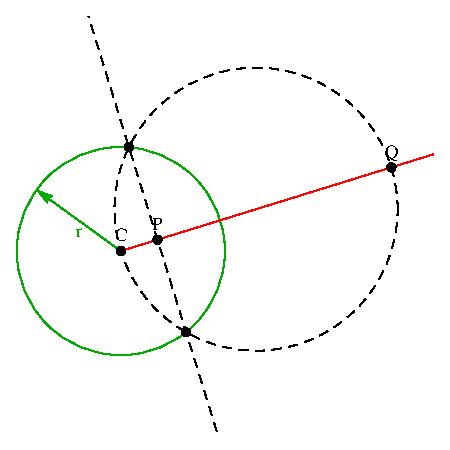
\includegraphics[width=0.5\textwidth]{figures/circ-inv}
\caption[Circle inversion]{Circle inversion with respect to the green reference circle. For a point $P$ within the reference circle the inverse $Q$ is constructed by first drawing a ray from $C$ through $P$ (red). The line normal to this ray through the point $P$ intersects the reference circle in two points. These two points together with $C$ determine a circle (dashed) which intersects the ray in the point $Q$.  The distances $CP$ and $CQ$ satisfy the relation $CP \cdot CQ = r^2$.}
\label{fig_CircInv}
\end{figure}

Coming back to the concrete map $z \mapsto \reci{z}$, it can now be interpreted the following way: Circle inversion with regard to the unit circle maps each $z \in \C$ to $\frac{z}{\abs{z}^2} = \reci{\conj{z}}$. Then reflection across the real axis (\ie complex conjugation) takes $\reci{\conj{z}}$ to $\reci{z}$. 

Summing up, all the basic types of M�bius transformations mentioned in Lemma \ref{lem_MoebiusGenerators} have a very direct geometric interpretation. Still, arbitrary M�bius transformations (especially those involving at least one inversion) are hard to describe in a similar geometric and intuitive way. Fortunately there is another characterization of M�bius transformations which is both, elegant and visually accessible.

% ---------------------------------------- Subsection: Stereographic projection
\subsection{Stereographic projection}

This section is about the great work of Douglas Arnold and Jonathan Rogness, ``M�bius transformations revealed'' \cite{arnold2008mobius}, in which the authors give a characterization of M�bius transformations in terms of stereographic projections and rigid motions of spheres 3D-space.

\todo{13}{Proof of characterization in terms of stereographic projection}


% --------------------------------------------- Subsection: Generalized circles
\subsection{Generalized circles}

\index{Generalized!circle}
From the geometric point of view M�bius transformations have the beautiful property that they preserve generalized circles. \emph{Generalized circles} are either circles (in the usual sense) or lines on the complex plane $\C$. They can also be thought of circles on the Riemann sphere (\ie the extended complex plane $\EC$ projected to the unit sphere $\UnitSphere$, see Remark~\ref{rem_RiemannSphere}), where lines on the complex plane stand in a one-to-one correspondence to circles through the point $\infty$ on the Riemann sphere. In order to give an exact definition, we follow an idea taken from \Schwerdtfeger{} and make the following considerations:

A circle with center $m \in \C$ and radius $r > 0$ can be described as the set of points $z \in \C$ for which
\begin{equation*}
\abs{z - m} = r.
\end{equation*}
This is obviously equivalent to
\begin{equation*}
\abs{z - m}^2 = (z - m) \conj{(z - m)} = r^2
\end{equation*}
and
\begin{equation}
\label{eqn_Circle}
z \conj{z} - m \conj{z} - \conj{m} z + m \conj{m} - r^2 = 0.
\end{equation}
The generalization comes into play if we multiply this last equation by a constant $A \in \R$
\begin{equation*}
A z \conj{z} - A m \conj{z} - A \conj{m} z + A m \conj{m} - A r^2 = 0
\end{equation*}
and introduce constants $B$, $C$ and $D$ appropriately such that we can write it in the form
\begin{equation}
\label{eqn_GenCircle}
A z \conj{z} + B \conj{z} + C z + D = 0.
\end{equation}
Note that $D$ is real and $B = \conj{C}$ are complex conjugates. From an equation of form (\ref{eqn_GenCircle}) we can read off the center and radius of the corresponding circle by
\begin{IEEEeqnarray}{rCl}
m &=& -\frac{B}{A}, \IEEEyessubnumber 
\label{eqn_GenCircCenter}\\
r &=& \sqrt{m \conj{m} - \frac{D}{A}} = \sqrt{\frac{BC - AD}{A^2}}. \IEEEyessubnumber 
\label{eqn_GenCircRadius}
\end{IEEEeqnarray}
Clearly we can only do so, if $A \ne 0$ and $BC - AD > 0$. 

In the case when $A = 0$, equation (\ref{eqn_GenCircle}) can be written as
\begin{equation*}
\Re{\frac{C}{\abs{C}} z} = -\frac{D}{2 \abs{C}},
\end{equation*}
which defines a line on the complex plane. We see this by considering the simpler equation $\Re{z} = -\frac{D}{2 \abs{C}}$ first (we omit the factor $\frac{C}{\abs{C}}$), which obviously defines a line parallel to the imaginary axis through the real point $-\frac{D}{2 \abs{C}}$. Then we observe that the multiplication with $\frac{C}{\abs{C}}$ just rotates this line around the origin by an angle which is given by $-\arg(C)$. 

Note that equation (\ref{eqn_GenCircle}) can also be written in matrix form:
\begin{equation*}
\rvec{\conj{z}}{1} \cdot \mat{A}{B}{C}{D} \cdot \cvec{z}{1} = 0.
\end{equation*}
If we substitute $z = u / v$, with $u,v \in \C$, $v \ne 0$ and scale by $\conj{v} \cdot v = \abs{v}^2 > 0$, we obtain the equivalent equation
\begin{equation}
\label{eqn_GenCircleMatForm}
\rvec{\conj{u}}{\conj{v}} \cdot \mat{A}{B}{C}{D} \cdot \cvec{u}{v} = 0.
\end{equation}
By introducing the convention to identify $\infty \in \EC$ with the formal quotient $u/0$, for arbitrary $u \in \C \setminus \{0\}$, equation (\ref{eqn_GenCircleMatForm}) makes sense for all $z = u/v \in \EC$. 

Finally we emphasize that the matrix in equation (\ref{eqn_GenCircleMatForm}) has a negative determinant, because of the condition $BC - AD > 0$ from above. Moreover it is a Hermitian matrix -- a notion which we will shortly recall:
\begin{definition}[Hermitian matrix]
\label{dfn_HermitianMatrix}
\index{Hermitian!matrix}
\index{Hermitian!transpose}
\index{Conjugate transpose}
Let $n > 0$ and $M \in \Mat{\C}{n}{n}$. The matrix
\begin{equation*}
\htransp{M} := \transp{\overline{M}}
\end{equation*}
obtained by complex conjugation and transposition of $M$ is called \emph{Hermitian transpose} or \emph{conjugate transpose} of $M$. If $M$ has the property $\htransp{M} = M$, it is called a \emph{Hermitian matrix}.
\end{definition}
Having now the right vocabulary and properties at hand, we can give an exact definition for generalized circles.
\begin{definition}[Generalized circle]
\index{G-circle}
\label{dfn_GenCircle}
Let $M \in \Mat{\C}{2}{2}$ be a Hermitian matrix with $\det(M) < 0$. A \emph{generalized circle}, for short \emph{g-circle}, is the set of solutions $u/v \in \EC$ with $u,v \in \C$, not both zero, to
\begin{equation}
\label{eqn_GenCircleDfn}
\rvec{\conj{u}}{\conj{v}} \cdot M \cdot \cvec{u}{v} = 0.
\end{equation}
\end{definition}

Since there should be no danger of confusion, we will from now on use the same name for a generalized circle and its corresponding Hermitian matrix (which is uniquely determined up to a nonzero real scalar factor).

\begin{remark}
Definition~\ref{dfn_GenCircle} does not depend on the choice of $u$ and $v$. If $u/v$ is a solution to (\ref{eqn_GenCircleDfn}) and $u^\prime/v^\prime = u/v$, \ie $u^\prime = \lambda u$ and $v^\prime = \lambda v$ for some $\lambda \in \C \setminus \{0\}$, then also
\begin{equation*}
\rvec{\conj{u^\prime}}{\conj{v^\prime}} \cdot M \cdot \cvec{u^\prime}{v^\prime} = \abs{\lambda}^2 \rvec{\conj{u}}{\conj{v}} \cdot M \cdot \cvec{u}{v} = 0.
\end{equation*}

Moreover we see that the point $\infty = 1/0$ lies on the g-circle $M = \smallmat{A}{B}{C}{D}$ exactly when its left upper matrix entry $A$ is zero. This is consistent with stereographic projection: The matrix entry $A$ is zero if and only if $M$ corresponds to a line on the complex plane. The image of this line under reverse stereographic projection is a circle on the Riemann sphere going through its north-pole, which we have identified with the point $\infty$.
\end{remark}

Going back to the our starting point, the equation $\abs{z - m} = r$, we can replace the equality sign `$=$' with `$<$' or `$\le$' and repeat the above considerations without any additional changes. This naturally leads to the notions of open and closed generalized disks.

\begin{definition}[Generalized disk]
\index{Generalized!disk}
\index{G-disk}
\label{dfn_GenDisk}
Let $M \in \Mat{\C}{2}{2}$ be a Hermitian matrix with $\det(M) < 0$. An \emph{open generalized disk} is the set of solutions $u/v \in \EC$, with $u,v \in \C$ -- not both zero, to
\begin{equation}
\label{eqn_GenOpenDiskDfn}
\rvec{\conj{u}}{\conj{v}} \cdot M \cdot \cvec{u}{v} < 0
\end{equation}
and a \emph{closed generalized disk} is the set of solutions $u/v \in \EC$ to
\begin{equation}
\label{eqn_GenClosedDiskDfn}
\rvec{\conj{u}}{\conj{v}} \cdot M \cdot \cvec{u}{v} \le 0.
\end{equation}
In both cases we will use the term (open/closed) \emph{g-disk} for shortness.
\end{definition}

\begin{remark}
In contrast to generalized circles, the defining matrix $M = \smallmat{A}{B}{C}{D}$ of a generalized disk is unique up to a \emph{positive} real scalar factor. Switching from $M$ to $-M$ turns the g-disk inside out while its border (the g-circle $M$) is left intact. Dependent on the sign of the left upper matrix entry $A$, we can distinguish three types of g-disks:
\begin{description}
\item[Case $A > 0$:] The g-disk corresponds to a disk in the usual sense within $\C$. Its center is given by (\ref{eqn_GenCircCenter}) and its radius by (\ref{eqn_GenCircRadius}).
\item[Case $A = 0$:] The g-disk corresponds to a half-plane of $\C$, which is obtained from the left half-plane, \ie $\Re{z} < 0$ (\resp $\le 0$), by translation by $\frac{-D}{2 \abs{C}}$ and rotation by $-\arg(C)$. The point $\infty$ is member of the generalized disk, if and only if it is closed.
\item[Case $A < 0$:] The open g-disk $M$ corresponds to the set complement (within $\EC$) of the closed g-disk $-M$ (discussed in the first case, $A > 0$). Accordingly, the closed g-disk $M$ is the complement of the open g-disk $-M$. Open and closed g-disks with $A < 0$ contain the point  $\infty$.
\end{description}
\end{remark}

It is now easy to show that g-circles and g-disks are preserved under M�bius transformations.

\begin{theorem}
\label{thm_MoebiusGenCircle}
Let $\phi$ be a M�bius transformation and $M \in \Mat{\C}{2}{2}$ be a Hermitian matrix with $\det(M) < 0$. The image of the g-circle (\resp open/closed g-disk) $M$ under the M�bius transformation $\phi$ corresponding to the matrix $P \in \GL{\C}$ is the g-circle (\resp open/closed g-disk)
\begin{equation}
\label{eqn_GDiskTransform}
\htransp{(\inv{P})} \cdot M \cdot \inv{P}.
\end{equation}
\end{theorem}
\begin{proof}
Let us write $P = \smallmat{a}{b}{c}{d}$, such that the corresponding M�bius transformation $\phi$ has the form
\begin{equation*}
\phi\left(\frac{u}{v}\right) = \frac{a u + b v}{c u + d v}.
\end{equation*}
Define $u^\prime := a u + b v$ and $v^\prime := c u + d v$. We need to show that
\begin{equation*}
\rvec{\conj{u}}{\conj{v}} \cdot M \cdot \cvec{u}{v} 
\ \left\{\ \begin{matrix} = 0 \\ < 0\\ \le 0 \end{matrix}\right.
\end{equation*}
if and only if
\begin{equation*}
\rvec{\conj{u^\prime}}{\conj{v^\prime}} \cdot \htransp{(\inv{P})} \cdot M \cdot \inv{P} \cdot \cvec{u^\prime}{v^\prime} 
\ \left\{\ \begin{matrix} = 0\phantom{.} \\ < 0\phantom{.}\\ \le 0. \end{matrix}\right.
\end{equation*}
But this follows immediately from
\begin{equation*}
P \cdot \cvec{u}{v} = \cvec{a u + b v}{c u + d v} = \cvec{u^\prime}{v^\prime}.\qedhere
\end{equation*}
\end{proof}




% ----------------------------------------------------- CHAPTER: THEORETIC PART
\chapter{The modular group and its subgroups}

% ------------------------------------------------------ Section: Modular group
\section{The modular group}

Throughout this section and also later, we adopt the notation of \Schoeneberg{}.

\begin{definition}
\label{dfn_ModularGroup}
\index{Modular!group}
\index{Modular!transformation}
\index{Inhomogeneous!modular transformation}
A M�bius transformation $\phi$ of the form
\begin{equation*}
\phi(z) = \moebius{a}{b}{c}{d}{z},\quad a,b,c,d \in \Z,\quad ad - bc = 1
\end{equation*}
is called \emph{(inhomogeneous) modular transformation}.
\end{definition}

\begin{theorem}
\label{thm_ModularGroup}
\index{Modular!group}
The set of modular transformations forms a discrete subgroup of the group of M�bius transformations and can be identified with the projective special linear group $\PSL{\Z}$. This group is called the \emph{modular group} and is denoted by $\ModGrp$.
\end{theorem}
\begin{proof}
The proof is very similar to that of Theorem \ref{thm_MoebiusGroup}. The only thing which has to be changed is the homomorphism $\pi$ defined in (\ref{eqn_homPi}). Its domain now is $\SL{\Z}$, the group of 2-by-2 matrices over $\Z$ with determinant 1, rather than $\GL{\C}$ (or $\SL{\C}$). Again it follows by the first isomorphism theorem, that the modular group $\ModGrp$ is isomorphic to $\SL{\Z} / \ker(\pi) \cong \PSL{\Z}$. The fact that $\ModGrp$ is a discrete subgroup of the group of M�bius transformations is now also directly evident.
\end{proof}

\begin{remark}
\index{Inhomogeneous!modular transformation}
\index{Homogeneous!modular transformation}
\index{Modular!transformation}
The elements of $\SL{\Z}$ are often called \emph{homogeneous modular transformations}, whereas the transformations of $\ModGrp = \PSL{\Z}$ are called \emph{inhomogeneous transformations}. Strictly seen, an inhomogeneous transformation has to be denoted as $[M]_{\sim}$, which is the equivalence class in $\PSL{\Z}$ of a matrix $M \in \SL{\Z}$. It is clear, that $[M]_{\sim}$ is nothing but the set $\{\pm M\}$ and again for easier notation, we will from now on simply write either $M$ or $-M$ instead of $[M]_{\sim}$. Additionally we will denote equivalence of matrices by $\sim$, \ie, if $\lambda = \pm 1$, then $M \sim \lambda M$.
\end{remark}

\todo{16}{Basic mapping properties}

\subsection{Generators and relations}
\label{sec_ModularGroupGenRel}

In group theory it is an important question, which systems of group elements and relations completely describe the structure of any given group (in the sense of Definition~\ref{dfn_GrpConstructGenRel}). This section is devoted to the investigation of this question in the case of the modular group.

Before we start, we introduce the following three important modular transformations which will be used very frequently from now on:

\begin{IEEEeqnarray*}{RL}
U: & z \mapsto z + 1 \\
T: & z \mapsto -\reci{z} \\
R = TU: & z \mapsto -\reci{z + 1}
\end{IEEEeqnarray*}

\begin{remark}
Unfortunately, in literature there is no consensus on the notation of these transformations. We use the notation of \Schoeneberg{} here, but other notations are frequent. For example in \Klein{}, the symbol $S$ is used instead of $U$ and in other literature as well as on Wikipedia, additionally the roles of $S$ and $T$ are swapped.
\end{remark}

\begin{theorem}
\label{thm_ModGrpTUGen}
The modular group is generated by the elements $U: z \mapsto z+1$ and $T: z \mapsto -\reci{z}$. 
\end{theorem}
\begin{proof}
Let $A: z \mapsto \moebius{a}{b}{c}{d}{z}$ be an arbitrary modular transformation. Our goal is to show that $A$ can be written as product of the transformations $U$ and $T$. For this purpose it is more convenient to view these transformations as elements of $\PSL{\Z}$, namely
\begin{equation*}
A = \mat{a}{b}{c}{d}, \quad U = \mat{1}{1}{0}{1}, \quad T = \mat{0}{-1}{1}{\phantom{+}0}.
\end{equation*}

Let's first consider the two special cases, when $a$ or $c$ are zero. If $a=0$, it follows from $ad - bc = 1$, that $-b = c = \pm 1$. Therefore we have (equivalence of matrices is again denoted by $\sim$)
\begin{equation*}
A \sim c A = \mat{0}{-1}{1}{c d} = TU^{c d}.
\end{equation*}
Similarly, $c = 0$ gives $a = d = \pm 1$ and
\begin{equation*}
A \sim a A = \mat{1}{a b}{0}{1} = U^{a b}.
\end{equation*}
In the more general case, when $a$ and $c$ are both nonzero, $ad - bc = 1$ implies that $a$ and $c$ are coprime and the Euclidean algorithm therefore yields
\begin{eqnarray*}
      a &=& q_0 \cdot c\phantom{_0} + r_1 \\
      c &=& q_1 \cdot r_1 + r_2 \\
    r_1 &=& q_2 \cdot r_2 + r_3 \\
        &\vdots& \\
r_{n-1} &=& q_n \cdot r_n + r_{n+1}\\
        &=& q_n \cdot 1\phantom{_n} + 0.
\end{eqnarray*}
We can use this to reduce the Matrix $A$ by successively multiplying powers of $U$ and $T$ from the left. Just note, that multiplication with $U^k$ adds $k$ times the second row to the first row, whereas $T$ swaps the rows and changes the sign of one arbitrary row\footnote{This freedom of choice is again due to the fact that the matrices $M$ and $-M$ represent the same element in $\PSL{\Z}$.}. If we concentrate only on the first column of $A$ and apply the first few transformations
\begin{equation*}
\cvec{a}{c}                           \overset{U^{-q_0}}{\longmapsto}
\cvec{r_1}{c\phantom{_1}}             \overset{T}{\mapsto} 
\cvec{\phantom{+}c\phantom{_1}}{-r_1} \overset{U^{q_1}}{\longmapsto}
\cvec{\phantom{+}r_2}{-r_1}           \overset{T}{\mapsto} 
\cvec{r_1}{r_2}                       \overset{U^{-q_2}}{\longmapsto}
\cvec{r_3}{r_2}                       \overset{T}{\mapsto}
\cvec{\phantom{+}r_2}{-r_3}           \mapsto \dots,
\end{equation*}
we soon recognize the general mapping rule, which is
\begin{IEEEeqnarray*}{rCll}
\cvec{\phantom{+}r_{j-1}}{\phantom{+}r_{j\phantom{+0}}} 
& \overset{TU^{-q_j}}{\longmapsto}
& \cvec{\phantom{+}r_{j\phantom{+0}}}{-r_{j+1}}
& \quad \text{for even } j \text{ and}\\
\cvec{\phantom{+}r_{j-1}}{-r_{j\phantom{+0}}}
& \overset{TU^{q_j}}{\longmapsto}
& \cvec{\phantom{+}r_{j\phantom{+0}}}{\phantom{+}r_{j+1}} 
& \quad \text{for odd } j.
\end{IEEEeqnarray*}
When we set $r_{-1} := a$ and $r_0 := c$, this rule is applicable for $0 \le j \le n$. Obviously the described procedure ends with
\begin{equation*}
\cdots \overset{T}{\mapsto}
\cvec{\phantom{+}r_{n\phantom{+0}}}{\pm r_{n+1}} = \cvec{1}{0}.
\end{equation*} 
Because we know the first column of the resulting matrix and its determinant, which is 1, we can conclude that for some $k \in \Z$ it must have the form
\begin{equation*}
\mat{1}{k}{0}{1} = U^k.
\end{equation*}
By setting $e_n := (-1)^{n} q_n$, we therefore have 
\begin{equation*}
TU^{-e_n} TU^{-e_{n-1}} \cdots TU^{-e_1}TU^{-e_0} A = U^k
\end{equation*}
or equivalently,
\begin{equation*}
A = U^{e_0} TU^{e_1} \cdots TU^{e_{n-1}} TU^{e_n} T U^k,
\end{equation*}
which gives the desired representation of $A$ in terms of $U$ and $T$ in the case when $a$ and $c$ are both nonzero.
\end{proof}

It is worth formulating the algorithm used in the previous proof explicitly in the following corollary.
\begin{corollary}
\label{cor_ModGrpTUAlg}
An arbitrary modular transformation $A: z \mapsto \moebius{a}{b}{c}{d}{z}$ can be represented as product of the transformations $U: z \mapsto z+1$ and $T : z \mapsto -\reci{z}$, by performing the following steps:
\begin{enumerate}
\item If $a = 0$, then $A = TU^{c d}$ and if $c = 0$, then $A = U^{a b}$ and we are done. Otherwise, continue with \ref{itm_ModGrpTUAlgStart}.
\item \label{itm_ModGrpTUAlgStart} Apply the Euclidean algorithm to $a$ and $c$ with the first division being $a = q_0 \cdot c + r_1$ ($q_0$ may be $\le 0$) and let $n$ be the number of the  last division (start counting from 0). Call the arising quotients $q_0,q_1,\dots,q_n$.
\item For $j \in \{0,1,\dots,n\}$ set $e_j := (-1)^j q_j$.
\item Calculate the matrix product $TU^{-e_n} TU^{-e_{n-1}} \cdots TU^{-e_1}TU^{-e_0} A$ and multiply by $\pm 1$ in order to obtain a representation with positive diagonal elements. Read off the right-upper entry and call it $k$.
\end{enumerate}
The transformation $A$ can now be written as
\begin{equation}
\label{eqn_ModGrpTUAlg}
A = U^{e_0} TU^{e_1} \cdots TU^{e_{n-1}} TU^{e_n} T U^k.
\end{equation}
\end{corollary}

We have seen that $T$ and $U$ generate the modular group, but it is not yet clear, which group words in $T$ and $U$ give the same modular transformations. For example, it is easy to see that $T^2 = 1$ and $(TU)^3 = 1$ are relations which are satisfied by $T$ and $U$. It is the goal of the following paragraphs to show that these two relations are in fact the only ones in the sense that all other relations are derived from these. We will do this by proving the following theorem:

\begin{theorem}
\label{thm_ModGrpTRProd}
Let $T: z \mapsto -\reci{z}$ and $R = TU: z \mapsto -\reci{z+1}$. Every modular transformation $A \in \ModGrp$ can be written uniquely in the form
\begin{equation}
\label{eqn_ModGrpTRProd}
A = R^{k_1} T R^{k_2} T \cdots R^{k_{n-1}} T R^{k_n} 
\end{equation}
with $n \in \N$, $k_2,\dots,k_{n-1} \in \{\pm 1\}$ and $k_1, k_n \in \{0, \pm 1\}$.
\end{theorem}

From the uniqueness of the product representation (\ref{eqn_ModGrpTRProd}) it follows, that we have in fact a \emph{presentation} of the modular group in the sense of Definition~\ref{dfn_GrpConstructGenRel}:

\begin{corollary}
\label{cor_ModGrpPresentation}
The modular group is generated by the elements $T: z \mapsto -\reci{z}$ and $R: z \mapsto -\reci{z+1}$ and can be presented as
\begin{equation}
\label{eqn_ModGrpPresentation}
\ModGrp \cong \presentation{T,R}{T^2 = R^3 = 1}.
\end{equation}
Therefore $\ModGrp$ is isomorphic to the free product of a cyclic group of order 2 and a cyclic group of order 3.
\end{corollary}
\begin{proof}
It is easy to see, that the relations $T^2 = R^2 = 1$ are indeed satisfied:
\begin{eqnarray*}
T^2 &=& \mat{0}{-1}{1}{\phantom{-}0}^2 = \mat{-1}{\phantom{-}0}{\phantom{-}0}{-1} \sim \mat{1}{0}{0}{1}, \\
R^3 &=& \mat{0}{-1}{1}{\phantom{+}1}^3 = \mat{-1}{\phantom{-}0}{\phantom{-}0}{-1} \sim \mat{1}{0}{0}{1}.
\end{eqnarray*}
Moreover, the elements of $\presentation{T,R}{T^2 = R^3 = 1}$ are precisely the group words of the form~(\ref{eqn_ModGrpTRProd}), as we have seen in Examples~\ref{ex_RTGroup} and \ref{ex_RTFreeProd}.
\end{proof}

Before we turn to the proof of Theorem~\ref{thm_ModGrpTRProd} we first make one helpful Definition and study its consequences.

\begin{definition}
\label{dfn_trsPredicates}
For a modular transformation $A: z \mapsto \moebius{a}{b}{c}{d}{z}$ we define the predicates $t$, $r$ and $s$ as well as a ``norm'' $n$:
\begin{IEEEeqnarray}{rCcCc}
\label{eqn_tpred}
t(A) &:\quad& ac \ge 0       &\quad\land\quad& bd \ge 0 \\
\label{eqn_rpred}
r(A) &:\quad& a^2 + ac \le 0 &\quad\land\quad& b^2 + bd \le 0 \\
\label{eqn_spred}
s(A) &:\quad& c^2 + ac \le 0 &\quad\land\quad& d^2 + bd \le 0
\end{IEEEeqnarray}
\begin{equation}
n(A) := a^2 + b^2 + c^2 + d^2.
\end{equation}
\end{definition}

Note, that $t$, $r$, $s$ and $n$ are well-defined, since they do not change their value if we switch from the matrix $A \in \PSL{\Z}$ to the equivalent matrix $-A$, \eg $t(A) \Leftrightarrow t(-A)$ and $n(A) = n(-A)$. Moreover, the predicates $t$, $r$, and $s$ partition the elements of the modular group into three classes:

\begin{lemma}
\label{lem_trsPartition}
Let $A: z \mapsto \moebius{a}{b}{c}{d}{z}$ be an arbitrary modular transformation. Then one, and only one of the predicates $t(A)$, $r(A)$ and $s(A)$ is satisfied.
\end{lemma}
\begin{proof}
We start by considering the two easiest cases first: If $A$ is the identity transformation or $A = T$, we have $t(A)$, $\lnot s(A)$ and $\lnot r(A)$.

For all other cases, we note that at least three of the coefficients $a,b,c,d$ are nonzero. Therefore, if one of the predicates $t(A)$, $r(A)$, $s(A)$ is satisfied, then at least one of the two inequalities involved is \emph{strictly} fulfilled. Having this said, it is easy to see that $t(A) \Rightarrow \lnot r(A) \land \lnot s(A)$. Thus it remains to show 
\begin{equation*}
\lnot t(A) \Rightarrow r(A) \lxor s(A),
\end{equation*}
for all transformations with at least three nonzero coefficients (here, $\lxor$ denotes logical exclusive or). If $t(A)$ is false, we have $ac < 0$ or $bd < 0$. Since both cases are completely symmetric, we may assume without restriction that $ac < 0$. Note, that $ac < 0$ and $ad - bc = 1$ implies $bd \le 0$ because otherwise if $bd > 0$, both terms $ad$ and $bc$ would have different nonzero signs and their difference could not be 1. We conclude the proof by distinguishing three cases:
\begin{description}
\item[Case $a^2 < c^2$:] From $ac < 0$ it follows that $a^2 + ac < 0\ (i)$ and $c^2 + ac > 0\ (ii)$. Additionally, from $ad - bc = 1$ we can conclude that $b^2 \le d^2$, because otherwise $\abs{ad}$ would differ from $\abs{bc}$ by more than 1. Therefore we also have $b^2 + bd \le 0\ (iii)$. Taking these pieces together, we have $(ii) \Rightarrow \lnot s(A)$ and $(i) \land (iii) \Rightarrow r(A)$.
\item[Case $a^2 > c^2$:] This case is complementary to the first one: Because of $ac < 0$ we have $a^2 + ac > 0\ (i)$ and $c^2 + ac < 0\ (ii)$. The equation $ad - bc = 1$ here implies $b^2 \ge d^2$ and $d^2 + bd \le 0\ (iii)$. Thus we have $(i) \Rightarrow \lnot r(A)$ and $(ii) \land (iii) \Rightarrow s(A)$.
\item[Case $a^2 = c^2$:] Note that this case is only possible with $a = -c = \pm 1$ (as $a$ and $c$ are coprime). Hence we have $a^2 + ac = c^2 + ac = 0$. However, $ad - bc = 1$ implies $b^2 \ne d^2$ and therefore we have $b^2 + bd \le 0 \lxor d^2 + bd \le 0$. So, also in this case we have $r(A) \lxor s(A)$.\qedhere
\end{description}
\end{proof}

We have not yet seen the real benefit and meaning of the predicates $t$, $r$ and $s$. The following lemma will imply that they do nothing but indicate the leftmost symbol in the unique $R$-$T$ product representation (\ref{eqn_ModGrpTRProd}) of $A$. To be precise, if we denote this leftmost symbol by $\alpha(A)$, we will see that $t(A) \Leftrightarrow \alpha(A) = T$, $r(A) \Leftrightarrow \alpha(A) = R$ and $s(A) \Leftrightarrow \alpha(A) = \inv{R}$. Moreover, we will show that the ``norm'' $n(A)$ grows monotonically with the number of symbols $R$ and $\inv{R}$ in the product representation of $A$.

\begin{lemma}
\label{lem_trsnRelations}
The predicates $t$, $r$, $s$ and the ``norm'' $n$ satisfy the following relations:
\begin{enumerate}[\qquad(i)]
\item $t(A) \Leftrightarrow r(RA) \Leftrightarrow s(\inv{R}A)$
\label{itm_trsPropA}
\item $\lnot t(A) \Rightarrow t(TA)$
\label{itm_trsPropB}
\item $n(A) = n(TA)$
\label{itm_trsPropC}
\item $t(A) \Rightarrow n(A) < n(RA) \land n(A) < n(\inv{R}A)$
\label{itm_trsPropD}
\end{enumerate}
\end{lemma}
\begin{proof}
For a better overview, we first write out the matrices corresponding to $TA$, $RA$ and $\inv{R}A$. Since $A = \smallmat{a}{b}{c}{d}$, $T = \smallmat{0}{-1}{1}{\phantom{-}0}$, $R = \smallmat{0}{-1}{1}{\phantom{+}1}$ and $\inv{R} = \smallmat{\phantom{+}1}{1}{-1}{0}$ these are:
\begin{equation*}
TA = \mat{-c}{-d}{\phantom{+}a}{\phantom{+}b},\quad RA = \mat{-c}{-d}{a+c}{b+d},\quad
\inv{R}A = \mat{a+c}{b+d}{-a}{-b}.
\end{equation*}
\begin{description}
\item[ad (\ref{itm_trsPropA}):] This is shown easily via two simple calculations:
\begin{IEEEeqnarray*}{rClCl}
r(RA)
&\Leftrightarrow& c^2 - c(a+c) \le 0 \land d^2 - d(b+d) \le 0 & &  \\
&\Leftrightarrow& ac \ge 0 \land bd \ge 0 &\Leftrightarrow& t(A) \\
s(\inv{R}A)
&\Leftrightarrow& a^2 - a(a+c) \le 0 \land b^2 - b(b+d) \le 0 & & \\
&\Leftrightarrow& ac \ge 0 \land bd \ge 0 &\Leftrightarrow& t(A)
\end{IEEEeqnarray*}
\item[ad (\ref{itm_trsPropB}):] We have already seen in the proof of Lemma~{\ref{lem_trsPartition}} that $\lnot t(A)$ implies $ac \le 0\ \land\ bd \le 0$ and one of these two inequalities is strictly satisfied. Therefore, also $t(TA): -ca \ge 0\ \land\ -db \ge 0$ is fulfilled.
\item[ad (\ref{itm_trsPropC}):] $n(A) = n(TA)$ is trivial.
\item[ad (\ref{itm_trsPropD}):] Note that $ad - bc = 1$ implies that always at least one of the numbers $a$ and $c$ (resp.\ $b$ and $d$) will be nonzero. Moreover, $t(A) \Rightarrow ac \ge 0 \land bd \ge 0$, and thus we have
\begin{IEEEeqnarray*}{+rCl+x*}
n(RA) - n(A)       &=& c^2 + 2ac + d^2 + 2bd > 0 \quad \text{and}\\
n(\inv{R}A) - n(A) &=& a^2 + 2ac + b^2 + 2bd > 0.&\qedhere
\end{IEEEeqnarray*}
\end{description}
\end{proof}

We can now formulate an algorithm, which yields a product representation of any arbitrary modular transformation in terms of the generators $R$ and $T$.

\begin{theorem}
\label{thm_ModGrpTRAlg}
For a modular transformation $A: z \mapsto \moebius{a}{b}{c}{d}{z}$, a product representation of the form (\ref{eqn_ModGrpTRProd}) can be found by performing the following steps:
\begin{enumerate}
\item Start with $k := 0$ and set $A_0 := A$.

\item If $A_k = 1$ go to step \ref{itm_ModGrpTRAlgFin}.
\label{itm_ModGrpTRAlgLoop}

\item Define $M_k$ as follows:
\label{itm_ModGrpTRAlgMDfn}
\begin{equation*}
t(A_k) \Rightarrow M_k := T,\quad
r(A_k) \Rightarrow M_k := R,\quad
s(A_k) \Rightarrow M_k := \inv{R}.
\end{equation*}

\item Set $A_{k+1} := M_k^{-1} A_k$, increment $k$ by one and continue with step \ref{itm_ModGrpTRAlgLoop}.
\label{itm_ModGrpTRAlgADfn}

\item If $k = 0$, $A = 1$ and the desired product representation is the empty product and otherwise it is $A = M_0 M_1 \cdots M_{k-1}$.
\label{itm_ModGrpTRAlgFin}
\end{enumerate}
\end{theorem}
\begin{proof}
First we observe, that the described algorithm yields a sequence of equations 
\begin{eqnarray*}
A_1 &=& M_0^{-1} A_0\\
A_2 &=& M_1^{-1} A_1\\
A_3 &=& M_2^{-1} A_2\\
    &\vdots&
\end{eqnarray*}
Note, that because of Lemma~\ref{lem_trsPartition}, the rule for the definition of the transformations $M_k$ from step \ref{itm_ModGrpTRAlgMDfn} is unambiguous. The relations (\ref{itm_trsPropA}) and (\ref{itm_trsPropB}) of Lemma~\ref{lem_trsnRelations} guarantee that for every pair of subsequent transformations $M_k$, $M_{k+1}$, one of them is $T$ and the other is either $R$ or $\inv{R}$. Additionally, the relations (\ref{itm_trsPropC}) and (\ref{itm_trsPropD}) imply $n(A_k) > n(A_{k+2})$. Since $n(1) = n(T) = 2$ is a lower bound for $n(A_k)$, the described procedure must terminate after a finite number $m$ of iterations and the product $A = M_0 M_1 \cdots M_{m-1}$ is indeed of the desired form (\ref{eqn_ModGrpTRProd}).
\end{proof}

Now have all tools in hand for the proof of Theorem~\ref{thm_ModGrpTRProd}. Note, that two alternative proofs can be found in \Schoeneberg{}, �4 and in \Klein{}, p.\ 452ff. 

\begin{proof}[Proof of Theorem \ref{thm_ModGrpTRProd}]
Let $A: z \mapsto \moebius{a}{b}{c}{d}{z}$ be an arbitrary modular transformation. The existence of a product representation of the form (\ref{eqn_ModGrpTRProd}) is ensured by the algorithm of Theorem~\ref{thm_ModGrpTRAlg}. In order to prove also its uniqueness, it is sufficient to show that the identity map has a unique product representation (namely the empty product). 

From the relations (\ref{itm_trsPropC}) and (\ref{itm_trsPropD}) of Lemma~\ref{lem_trsnRelations} we see that any product $P$ of the form (\ref{eqn_ModGrpTRProd}) containing at least one factor $R$ or $\inv{R}$ has a ``norm'' $n(P) > n(1) = 2$ and therefore $P \ne 1$. The only products which are free of factors $R$ and $\inv{R}$ are T and the empty product. Since $T \ne 1$, the identity map can indeed only be represented by the empty product. \qedhere
\end{proof}

We conclude this section with the final remark that algorithm~\ref{thm_ModGrpTRAlg} successively reduces a given matrix $A \in \PSL{\Z}$ by multiplication from the left with $T$, $R$ or $\inv{R}$. Of course, by using a dual approach also multiplication from the right can be used. All we have to do in order to adapt algorithm~\ref{thm_ModGrpTRAlg} appropriately is to substitute the predicates $t$, $r$, $s$ by predicates $t^{\prime}$, $r^{\prime}$, $s^{\prime}$ and to change the definition in step \ref{itm_ModGrpTRAlgADfn} from $A_{k+1} := M_k^{-1} A_k$ to $A_{k+1} := A_k M_k^{-1}$. But how do the predicates $t^{\prime}$, $r^{\prime}$ and $s^{\prime}$ have to be defined?

For this consideration we denote the leftmost symbol in the $R$-$T$ product representation (\ref{eqn_ModGrpTRProd}) of $A$ by $\alpha(A)$ and the rightmost symbol by $\omega(A)$. In the case of the empty product, we define $\alpha(1) := \omega(1) := T$. We have already seen, that $t(A) \Leftrightarrow \alpha(A) = T$, $r(A) \Leftrightarrow \alpha(A) = R$ and $s(A) \Leftrightarrow \alpha(A) = \inv{R}$. In correspondence to that, we see that we have to define 
\begin{IEEEeqnarray*}{RrClCrClCc}
t^{\prime}(A):\quad& \omega(A) &=& T 
              &\quad\Leftrightarrow\quad& \alpha(\inv{A}) &=& T
              &\quad\Leftrightarrow\quad& t(\inv{A}), \\
r^{\prime}(A):\quad& \omega(A) &=& R 
              &\quad\Leftrightarrow\quad& \alpha(\inv{A}) &=& \inv{R}
              &\quad\Leftrightarrow\quad& s(\inv{A}), \\
s^{\prime}(A):\quad& \omega(A) &=& \inv{R}
              &\quad\Leftrightarrow\quad& \alpha(\inv{A}) &=& R
              &\quad\Leftrightarrow\quad& r(\inv{A}).
\end{IEEEeqnarray*}
Written out explicitly, this gives for a matrix $A = \smallmat{a}{b}{c}{d} \in \PSL{\Z}$:
\begin{IEEEeqnarray}{rCcCc}
\label{eqn_trpred}
t^{\prime}(A) &:\quad& ab \le 0       &\quad\land\quad& cd \le 0 \\
\label{eqn_rrpred}
r^{\prime}(A) &:\quad& a^2 - ab \le 0 &\quad\land\quad& c^2 - cd \le 0 \\
\label{eqn_srpred}
s^{\prime}(A) &:\quad& b^2 - ab \le 0 &\quad\land\quad& d^2 - cd \le 0
\end{IEEEeqnarray}
Note, that also the Lemmas \ref{lem_trsPartition} and \ref{lem_trsnRelations} remain valid, if the predicates $t$, $r$, $s$ are substitued by $t^{\prime}$, $r^{\prime}$, $s^{\prime}$ and the order of matrix multiplication is reversed (\ie $RA$, $TA$, \dots\ have to be replaced by $AR$, $AT$, \dots).

% ------------------------------- Subsection: Fundamental domains, tessellation
\subsection{The fundamental domain and the tessellation of the halfplane}

We have seen in Remark~\ref{rem_NatureMoebius} that considering M�bius transformations as meromorphic functions $\EC \to \EC$ very naturally induces a group action of $\PGL{\C}$ on $\EC$. Clearly this group action is also given for any subgroup of $\PGL{\C}$ and in particular for the modular group. 

For the following it will turn out useful to write modular transformations in matrix form and the elements $z \in \EC$ as quotients $z = u/v$ for suitable $u,v \in \C$, not both zero. A formal quotient $u/0$ will be identified with $\infty$. In this notation, for a modular transformation $A = \smallmat{a}{b}{c}{d} \in \PSL{\Z}$ and $u/v \in \EC$ the mentioned group action is given by
\begin{equation}
\label{eqn_ModGrpAction}
A \ \frac{u}{v} := \frac{a u + b v}{c u + d v}
\end{equation}
We call two points $z, w \in \EC$ \emph{equivalent}, if and only if there is a modular transformation $A \in \PSL{\Z}$ with $A z = w$ and we write  $z \sim w$. The equivalence class (\emph{orbit}) of a point $u/v \in \EC$ is given by 
\begin{equation*}
\left[\frac{u}{v}\right]_\sim = 
\setdefsz{\bigg}{\frac{a u + b v}{c u + d v} \in \EC}{\mat{a}{b}{c}{d} \in \PSL{\Z}} \in \EC / \sim.
\end{equation*}

We now wish to find a system of representatives for $\EC/\sim$, in other words, we want to define exactly one representative $u_0/v_0$ for each orbit $[u/v]_\sim$. One approach for this could be to fix $u,v \in \C$, not both zero, then to choose from the set
\begin{equation}
\label{eqn_FunDomOuv}
O_{u,v} := \SL{\Z} \cvec{u}{v} = \setdefsz{\bigg}{\cvec{a u + b v}{c u + d v} \in \C^2}{\mat{a}{b}{c}{d} \in \SL{\Z}}
\end{equation}
one vector $(u_0, v_0)$ with minimal $\eucnorm{\cdot}$-norm\footnote{We equip $\C^2$ with the standard Euclidean norm: $\eucnorm{\cvec{u}{v}} := \sqrt{\abs{u}^2 + \abs{v}^2}$.} and to declare $u_0/v_0$ as the representative for $[u/v]_\sim$. The problem with this is that such a choice may not always be possible, because $O_{u,v}$ may in general contain vectors of arbitrary small $\eucnorm{\cdot}$-norm. 

However, if $u \conj{v} \notin \R$, then $u$ and $v$ are linear independent over $\R$ and therefore span a non-degenerate parallelogram $P_{u,v} := \setdef{t u + s v}{t,s \in [0,1)} \subseteq \C$. Translation of $P_{u,v}$ by integer multiples of $u$ and $v$ covers every point in $\C$ exactly once. The set
\begin{equation*}
L_{u,v} := \setdef{a u + b v \in \C}{a,b \in \Z}
\end{equation*}
consists precisely of the vertices of all of these translated parallelograms. If we denote by $D_r := \setdef{z \in \C}{\abs{z} \le r}$ a disk of radius $r$ centered at the origin, then for every $r > 0$ the set $D_r \cap L_{u,v}$ is obviously finite. It follows that the set $O_{u,v} \subseteq (L_{u,v})^2$ must contain an element of minimal $\eucnorm{.}$-norm: Define $K_r := \setdef{x \in \C^2}{\eucnorm{x} \le r}$ and let $r > 0$ be sufficiently large such that $K_r \cap O_{u,v}$ is nonempty. Because 
\begin{equation}
\label{eqn_FunDomOuvFinite}
K_r \cap O_{u,v} \subseteq (D_r \cap L_{u,v})^2,
\end{equation}
we see that $K_r \cap O_{u,v}$ is finite and $\min \eucnorm{K_r \cap O_{u,v}} = \min \eucnorm{O_{u,v}}$ exists. Since $(0,0) \notin O_{u,v}$, this minimum is not zero.

This encourages us to go on (we will come back to the case $u \conj{v} \in \R$ later) and turn to the question, how we can effectively determine an element of $O_{u,v}$ with minimal $\eucnorm{\cdot}$-norm. The task is the following: Given two complex numbers $u,v \in \C$ with $u \conj{v} \notin \R$, find a matrix $B \in \SL{\Z}$ such that $\eucnorm{B ({}^u_v)}$ is minimal. 

In Corollary~\ref{cor_SLZandPSLZGen} we have seen that $\SL{\Z}$ is generated by the matrices $T = \smallmat{0}{-1}{1}{\phantom{-}0}$ and $U = \smallmat{1}{1}{0}{1}$. The idea is now to successively multiply $({}^u_v)$ with appropriate powers of $T$ and $U$ to obtain vectors of smaller and smaller $\eucnorm{\cdot}$-norm. We do this by first finding an integer $k_0 \in \Z$, such that $\eucnorm{U^{-k_0} ({}^u_v)}$ is minimal. Then we multiply with $T$ and repeat the process for finding $k_1 \in \Z$ minimizing $\eucnorm{U^{k_1} T U^{k_0} ({}^u_v)}$ and so on. The procedure ends when $k_n = 0$ for some $n>0$. Note that the integers $k_j$ can be determined easily:
\begin{lemma}
\label{lem_FunDomUVMin}
Let $u,v \in \C$ with $v \ne 0$. The statements
\begin{enumerate}[\qquad(i)]
\item \label{itm_uvMini}
$k \in \Z$ minimizes $\eucnorm{U^{-k}\cvec{u}{v}} = \eucnorm{\cvec{u - k v}{v}}$,
\item \label{itm_uvMinii} $k \in \Z$ minimizes $\abs{u - k v}$,
\item \label{itm_uvMiniii} $k \in \Z$ minimizes $\abs{\frac{u}{v} - k}$,
\item \label{itm_uvMiniv} $k = \nint{\Re{\frac{u}{v}}}$,
\end{enumerate}
satisfy the relations $(\ref{itm_uvMini}) \Leftrightarrow (\ref{itm_uvMinii}) \Leftrightarrow (\ref{itm_uvMiniii})$ and $(\ref{itm_uvMiniv}) \Rightarrow (\ref{itm_uvMiniii})$.
\end{lemma}
\begin{proof}
The equivalence of statements (\ref{itm_uvMini}), (\ref{itm_uvMinii}) and (\ref{itm_uvMiniii}) is directly evident. For minimizing $\abs{\frac{u}{v} - k}$ it is clear that $k$ has to be chosen as close as possible to $\Re{\frac{u}{v}}$, \ie $\abs{\Re{\frac{u}{v}} - k} \le \reci{2}$, which is certainly true for (\ref{itm_uvMiniv}).
\end{proof}

Let us now suppose that the described procedure comes to an end, \ie $k_n = 0$ for some $n > 0$. Set $B  := TU^{k_{n-1}} \cdots TU^{k_0}$ and $x := ({}^{u_0}_{v_0}) := B ({}^u_v)$. It follows from $k_n = 0$ and from the choice of $k_{n-1}$ that we have 
\begin{equation}
\label{eqn_FunDomUVLokMin}
\eucnorm{x} \le \eucnorm{U^k x} \text{\quad and \quad} \eucnorm{x} \le \eucnorm{U^k \inv{T} x} \text{\quad for all } k \in \Z.
\end{equation}
Using similar arguments as in Lemma~\ref{lem_FunDomUVMin}, we see that (\ref{eqn_FunDomUVLokMin}) is equivalent to
\begin{equation*}
\abs{\Re{\frac{u_0}{v_0}}} \le \reci{2} \text{\quad and \quad} \abs{\Re{\frac{v_0}{u_0}}} \le \reci{2}.
\end{equation*}
Note that this can easily be rewritten to
\begin{equation*}
u_0 \conj{v_0} + \conj{u_0} v_0 \le \min\{\abs{u_0}^2, \abs{v_0}^2\}.
\end{equation*}
The question arises, if $x = ({}^{u_0}_{v_0})$ is just a ``local minimum'' in the sense (\ref{eqn_FunDomUVLokMin}) or if the above conditions are already sufficient for the global minimality of $x$, \ie $\eucnorm{x} = \min \eucnorm{O_{u,v}}$. The following Lemma will give us an answer on this.

\begin{lemma}
\label{lem_FunDomUVGlobMin}
Let $A \in \SL{\Z}$ and the \emph{grading} $n(A)$ be defined as in (\ref{eqn_grading}). Let $x = ({}^u_v) \in \C^2$ be a vector with $0 \notin \{u,v\}$. Then the following statements hold:
\begin{enumerate}[(i)]
\item \label{itm_FunDomUVGlobMinA}
If $\abs{u\conj{v} + \conj{u}v} \le \min\{\abs{u}^2,\abs{v}^2\}$, then $\eucnorm{x} \le \eucnorm{Ax}$.
\item \label{itm_FunDomUVGlobMinB}
If $\abs{u\conj{v} + \conj{u}v} \le \min\{\abs{u}^2,\abs{v}^2\}$ and $n(A) > 3$, then $\eucnorm{x} < \eucnorm{Ax}$.
\item \label{itm_FunDomUVGlobMinC}
If $\abs{u\conj{v} + \conj{u}v} < \min\{\abs{u}^2,\abs{v}^2\}$ and $n(A) > 2$, 
then $\eucnorm{x} < \eucnorm{Ax}$.
\end{enumerate}
\end{lemma}
\begin{proof}
Let us denote $A = \smallmat{a}{b}{c}{d}$. We need to show $\eucnorm{x} \le \eucnorm{Ax}$, that is
\begin{eqnarray*}
\abs{u}^2 + \abs{v}^2 
&\le& \abs{au + bv}^2 + \abs{cu + dv}^2 =\\
&& (au + bv)(a\conj{u} + b\conj{v}) + (cu + dv)(c\conj{u} + d\conj{v}) =\\
&& (a^2 + c^2)\abs{u}^2 + (b^2 + d^2)\abs{v}^2 + (ab + cd)(u\conj{v} + \conj{u}v),
\end{eqnarray*}
which is equivalent to
\begin{equation*}
(a^2 + c^2 - 1)\abs{u}^2 + (b^2 + d^2 - 1)\abs{v}^2 \ge -(ab + cd)(u\conj{v} + \conj{u}v).
\end{equation*}
Now we find an upper bound of the right hand side by taking its absolute value and using $\abs{u\conj{v} + \conj{u}v} \le \min\{\abs{u}^2, \abs{v}^2\} =: m$. The same time, $m$ also helps us with a lower bound of the left hand side:
\begin{equation*}
(a^2 + b^2 + c^2 + d^2 - 2) \cdot m \ge \abs{ab + cd} \cdot m.
\end{equation*}
Since $m$ is nonzero ($u,v \ne 0$), it can be canceled. Moreover, $ad - bc = 1$ implies that the terms $ad$ and $bc$ can never have opposite signs. In other words we always have $(ad)(bc) \ge 0$. Obviously also $(ab)(cd) \ge 0$, \ie also the terms $ad$ and $bc$ have non-opposite signs, which is why $\abs{ab + cd} = \abs{ab} + \abs{bd}$. Therefore we can transform the last inequality to
\begin{equation}
\label{eqn_FunDomUVIneq}
\underbrace{(a^2 - \abs{ab} + b^2)}_{\ge(\abs{a}-\abs{b})^2 =: \ell} + 
\underbrace{(c^2 - \abs{cd} + d^2)}_{\ge(\abs{c}-\abs{d})^2 =: r} \ge 2.
\end{equation}
This obviously holds for the case $n(A) = 2$. For the case $n(A) > 2$, because of $ad - bc = 1$, we see:
\begin{enumerate}[\quad(a)]
\item 
\label{itm_FunDomUVObsA}
$\abs{a} = \abs{b}$ implies $\abs{c} \ne \abs{d}$ (and vice versa). Therefore at least one of the lower bounds $\ell$ and $r$ is nonzero.
\item 
\label{itm_FunDomUVObsB}
$\abs{ab} = 0$ implies $\abs{bc} \ne 0$ (and vice versa). Therefore at least one of the lower bounds $\ell$ and $r$ is in fact a \emph{strict} lower bound.
\end{enumerate}
These two observations prove (\ref{eqn_FunDomUVIneq}) and consequently assertion (\ref{itm_FunDomUVGlobMinA}). If additionally $n(A) > 3$, we distinguish two cases:
\begin{description}
\item[Case $0 \in \{a,b,c,d\}$:] Assume without restriction that $0 \in \{a,b\}$, (the case $0 \in \{c,d\}$ is completely symmetric). It follows $\{\abs{a},\abs{b}\} = \{0,1\}$ and $\{\abs{c},\abs{d}\} = \{1,N\}$ with $N > 1$, since $n(A) > 3$. Therefore, in addition to observation (\ref{itm_FunDomUVObsB}), both lower bounds $\ell$ and $r$ are positive. 
\item[Case $0 \notin \{a,b,c,d\}$:] In addition to observation (\ref{itm_FunDomUVObsA}), $\abs{ab}$ and $\abs{cd}$ are nonzero. Therefore $\ell$ and $r$ are both strict lower bounds.
\end{description}
In both cases (\ref{eqn_FunDomUVIneq}) is strictly fulfilled, which proves (\ref{itm_FunDomUVGlobMinB}). For proving (\ref{itm_FunDomUVGlobMinC}) it is sufficient to consider the special case $n(A) = 3$, as the assumption for the case $n(A) > 3$ is already implied by (\ref{itm_FunDomUVGlobMinB}). By the same arguments as above, $\eucnorm{x} < \eucnorm{Ax}$ is equivalent to
\begin{equation}
\label{eqn_FunDomUVIneqB}
(a^2 + c^2 - 1)\abs{u}^2 + (b^2 + d^2 - 1)\abs{v}^2 > -(ab + cd)(u\conj{v} + \conj{u}v).
\end{equation}
For $n(A) = 3$ we have $\{(a^2 + c^2 - 1),(b^2 + d^2 - 1)\} = \{0,1\}$, which means that the left hand side simplifies to either $\abs{u}^2$ or $\abs{v}^2$, whereas on the right hand side we have $\abs{u\conj{v} + \conj{u}v}$ as upper bound, because of $(ab + cd) = \pm 1$. Since $\abs{u\conj{v} + \conj{u}v} < \min\{\abs{u}^2,\abs{v}^2\}$, inequality (\ref{eqn_FunDomUVIneqB}) is thus satisfied.
\end{proof}

In the following theorem we summarize the described algorithm and prove its correctness:

\begin{theorem}
\label{thm_FunDomUVAlg}
Let $u,v \in \C$ with $u \conj{v} \notin \R$. A matrix $B \in \SL{\Z}$ minimizing $\eucnorm{B ({}^u_v)}$ can be found by performing the following steps:
\begin{enumerate}
\item Set $(r_{-1},r_0) := (u,v)$ and $j := 0$.
\item \label{itm_FunDomUVAlgLoop}
Determine $q_j := \nint{\Re{\frac{r_{j-1}}{r_j}}}$.
\item If $j > 0$ and $q_j = 0$ go to step \ref{itm_FunDomUVAlgDone}. Otherwise, set $r_{j+1} := r_{j-1} - q_j r_j$, increment $j$ by one and continue with step \ref{itm_FunDomUVAlgLoop}.
\item \label{itm_FunDomUVAlgDone} Set $n := j-1$. For $i \in \{0,1,\dots,n\}$, set $e_i := (-1)^i q_i$. The desired matrix is
\begin{equation}
\label{eqn_FunDomUVMinMat}
B = U^{-e_n} TU^{-e_{n-1}} \cdots TU^{-e_0}.
\end{equation}
\end{enumerate}
\end{theorem}
\begin{proof}
The algorithm gives rise to a sequence of equations
\begin{IEEEeqnarray*}{rCcCl}
u &=& r_{-1} &=& q_0 \cdot r_0 + r_1 \\
v &=&    r_0 &=& q_1 \cdot r_1 + r_2 \\
&&       r_1 &=& q_2 \cdot r_2 + r_3 \\
&&       r_2 &=& q_3 \cdot r_3 + r_4 \\
&& &\vdots& 
\end{IEEEeqnarray*}
with $r_j \ne 0$ for all $j \ge -1$, because they are all nontrivial linear combinations of $u$ and $v$ with integer coefficients and $u\conj{v} \notin \R$ implies linear independence of $u$, $v$ over $\R$.  Moreover this sequence of equations corresponds to the sequence of vectors
\begin{equation*}
\cvec{u}{v}                           \overset{TU^{-q_0}}{\longmapsto}
\cvec{\phantom{+}v\phantom{_1}}{-r_1} \overset{TU^{q_1}}{\longmapsto}
\cvec{-r_1}{-r_2}                     \overset{TU^{-q_2}}{\longmapsto}
\cvec{-r_2}{\phantom{+}r_3}           \overset{TU^{q_3}}{\longmapsto}
\cvec{r_3}{r_4}                       \mapsto \dots
\end{equation*}
With $s_j := (-1)^{\ceil{\half{j}}} r_j$, we can write these vectors as $x_j := \cvec{s_{j-1}}{s_j}$ for $j \ge 0$. Now, as in the theorem, let $e_j := (-1)^j q_j$ for $j \ge 0$. In this notation, we can write in general $TU^{-e_j} x_j = x_{j+1}$ for all $j \ge 0$. From the choice of $q_j$ -- see Lemma~\ref{lem_FunDomUVMin} -- it follows that for each pair of subsequent vectors $x_j$, $x_{j+1}$ we have $\eucnorm{x_j} \ge \eucnorm{x_{j+1}}$. Using $r_{j+1} = r_{j-1} - q_j r_j$ we see that $\eucnorm{x_j} = \eucnorm{x_{j+1}}$ is equivalent to
\begin{equation*}
\eucnorm{\cvec{\pm r_{j-1}}{\pm r_{j\phantom{-1}}}} = 
\eucnorm{\cvec{\pm r_{j\phantom{+1}}}{\pm r_{j+1}}} =
\eucnorm{\cvec{\pm r_j}{\pm (r_{j-1} - q_j r_j)}}.
\end{equation*}
Obviously this is the case if and only if $\abs{r_{j-1}} = \abs{r_{j-1}-q_j r_j}$. If we divide by $r_j$ and define $z_j := \frac{r_{j-1}}{r_j}$, we obtain
\begin{eqnarray*}
\abs{z_j} = \abs{z_j - q_j} 
&\Leftrightarrow& z_j \conj{z_j} = (z_j - q_j)(\conj{z_j} -q_j)\\
&\Leftrightarrow& q_j \left(q_j - 2\Re{z_j}\right) = 0.
\end{eqnarray*}
One obvious solution to this is $q_j = 0$. For the other factor, we substitute $\alpha := \Re{z_j}$ and use $q_j = \nint{\alpha}$ to see that the equation $\nint{\alpha} = 2 \alpha$ has the unique\footnote{Here we benefit from our definition of $\operatorname{nint}$, which rounds $\pm \reci{2}$ to zero.} solution $\alpha = 0$ which again leads to $q_j = 0$. Summing up, we therefore have for all $j \ge 0$
\begin{equation}
\label{eqn_FunDomUVAlgNormDec}
\eucnorm{x_j} \ge \eucnorm{x_{j+1}} 
\quad \text{and} \quad
\eucnorm{x_j} = \eucnorm{x_{j+1}} \Leftrightarrow q_j = 0.
\end{equation}

To see that the algorithm terminates, let $O_{u,v}$ and $K_r$ be defined as in (\ref{eqn_FunDomOuv}) and (\ref{eqn_FunDomOuvFinite}). Since all the vectors $x_j$ are contained in the finite set $O_{u,v} \cap K_{\eucnorm{({}^u_v)}}$, we cannot have $\eucnorm{x_j} > \eucnorm{x_{j+1}}$ for infinitely many indices $j$. In other words, $q_n$ must be zero for some $n \in \N$ and we have
\begin{equation*}
TU^{-e_n} \cdots TU^{-e_1} TU^{-e_0} x_0 = x_n.
\end{equation*}
Since the vector $x_n$ satisfies (\ref{eqn_FunDomUVLokMin}), we can apply Lemma~\ref{lem_FunDomUVGlobMin} to see that $x_n$ has minimal $\eucnorm{\cdot}$-norm in $O_{u,v}$. Obviously also the vector $\inv{T}x_n$ has this property and we may therefore define $B$ as in ($\ref{eqn_FunDomUVMinMat}$).
\end{proof}

\begin{figure}
\centering
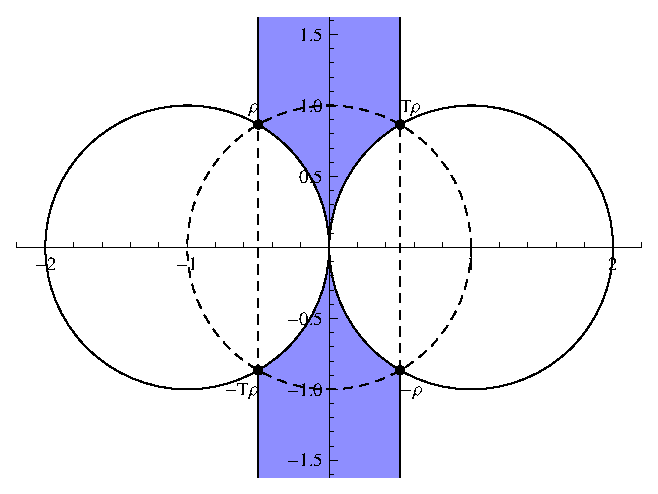
\includegraphics[width=0.8\textwidth]{figures/minimal-region}
\caption{The region of numbers $z \in \EC$, where $\Re{z}$ and $\Re{\reci{z}}$ are both contained in the interval $\left[-\half{1},\half{1}\right]$ is obtained by taking the strip $\Re{z} \in \left[-\half{1},\half{1}\right]$ and cutting out two disks of unit radius centered about the real points $\pm 1$. The arising vertices are labeled. As usual, $T$ is the transformation $z \mapsto -\reci{z}$ and $\rho = \exp(2 \pi \ii / 3)$ is a third root of unity.}
\label{fig_MinimalRegion}
\end{figure}

\begin{figure}
\centering
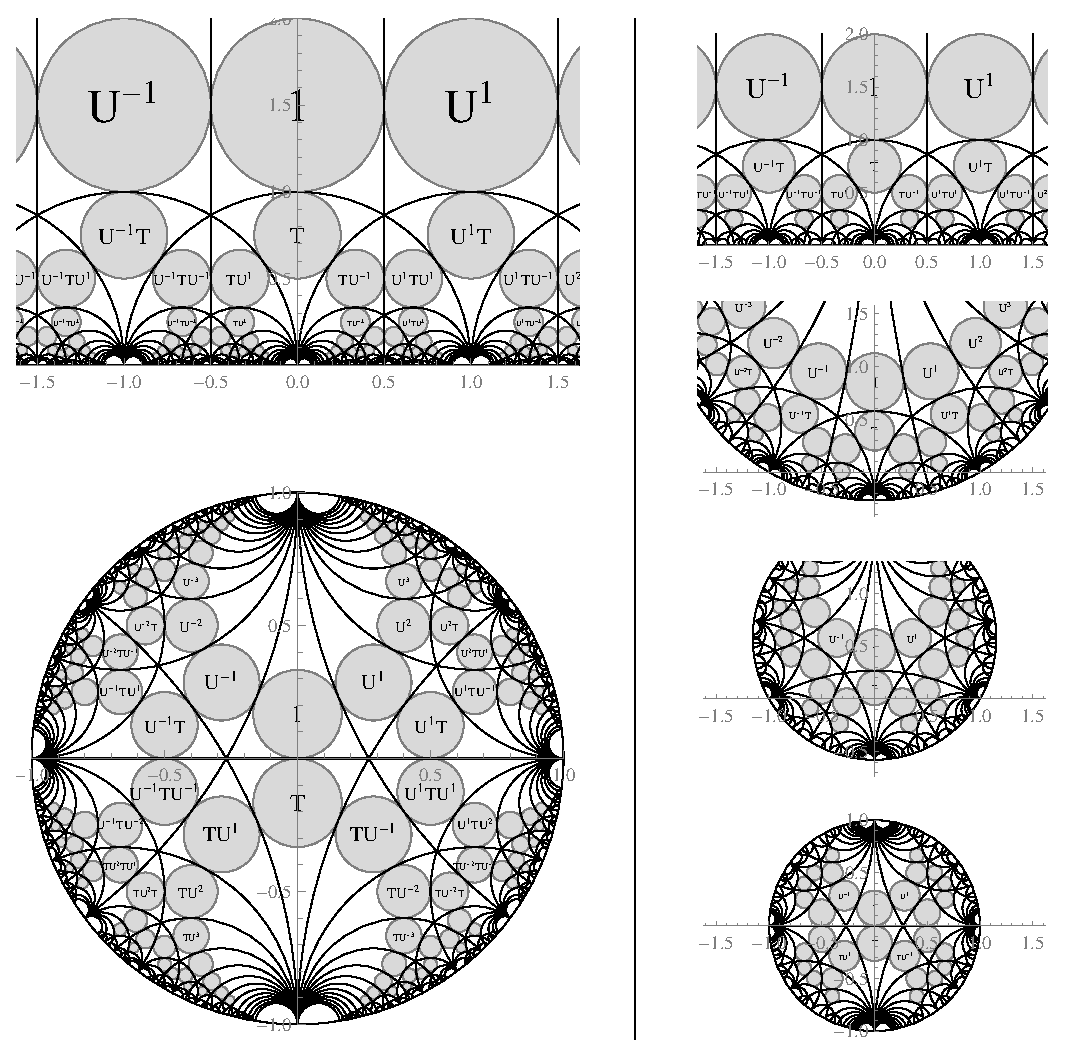
\includegraphics[width=\textwidth]{figures/modular-tiling-1}
\caption{The tessellation of the upper halfplane.}
\label{fig_ModularTiling}
\end{figure}

\begin{figure}
\centering
\includegraphics[width=0.8\textwidth]{figures/modular-tiling-exp-fan}
\caption{The tessellation under the transformation $z \mapsto \exp(2 \pi \ii z)$.}
\label{fig_ModularTilingExpFan}
\end{figure}

\begin{figure}
\centering
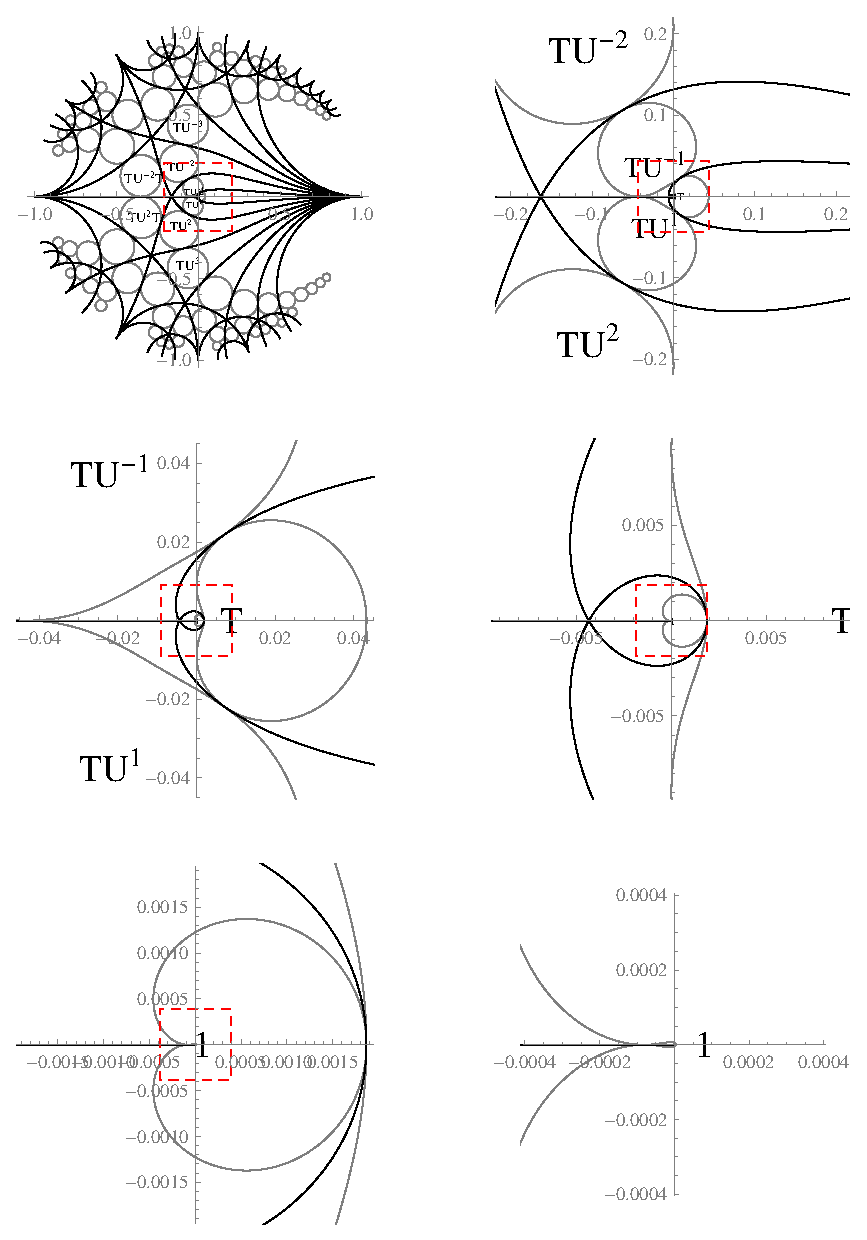
\includegraphics[width=0.8\textwidth]{figures/modular-tiling-exp-zoom}
\caption{The image of the modular tiling under the map $z \mapsto \exp(2 \pi \ii z)$ in the neighborhood of $\infty$.}
\label{fig_ModularTilingExpZoom}
\end{figure}


% --------------------------------------------- Subsection: Hyperbolic geometry
\subsection{Hyperbolic geometry}

\todo{11}{Connection to hyperbolic geometry (disk/halplane model)}


% ------------------------------- Subsection: Ford circles, continued fractions
\subsection{Ford circles and continued fractions}

For an arbitrary modular transformation $A$, a representation as product of shifts $U^j: z \mapsto z+j$ and inversions $T: z \mapsto -\reci{z}$ can be found by the algorithm described in Corollary \ref{cor_ModGrpTUAlg}. By writing out this product, for example in the case, when $n=2$, we have
\begin{equation*}
A = U^{e_0}T U^{e_1}T U^{e_2}T U^k,
\end{equation*}
or more explicitly
\begin{equation}
\label{eqn_ALongConFrac}
A(z) = e_0 - \reci{e_1 - \reci{e_2 - \reci{k + z}}}.
\end{equation}
\index{Continued fraction}
Here, a close relation between modular transformations and continued fractions immediately gets apparent. In this section, we will investigate this relation somewhat deeper. 
First, we will use Pringsheim's more space-saving notation for continued fractions, namely
\begin{equation}
\label{eqn_ConFracNotation}
b_0 + \frac{a_1}{b_1 + \frac{a_2}{b_2 + \frac{a_3}{b_3 + \dots}}} =: 
b_0 + \cfr{a_1}{b_1} + \cfr{a_2}{b_2} + \cfr{a_2}{b_3} + \dots
\end{equation}
In the case when all $a_j = 1$, we adhere to the standard sequence notation for continued fractions:
\begin{equation*}
b_0 + \reci{b_1 + \reci{b_2 + \dots}} =: [b_0,b_1,b_2,\dots].
\end{equation*}
We can now reformulate Corollary \ref{cor_ModGrpTUAlg} in order to construct a continued fraction representation of any given modular transformation.

\begin{corollary}
An arbitrary modular transformation $A(z) = \moebius{a}{b}{c}{d}{z}$ can be written as continued fraction
\begin{equation}
\label{eqn_ModTransConFrac}
A(z) = [q_0,q_1,\dots,q_n,(-1)^{n+1}(k+z)]
\end{equation}
where the integers $n$, $q_0,q_1,\dots,q_n$ and $k$ are determined by the algorithm described in Corollary \ref{cor_ModGrpTUAlg}.
\end{corollary}
\begin{proof}
By using the continued fraction representation of $A$ given in (\ref{eqn_ALongConFrac}) and by applying the definition $e_j$ := $(-1)^j q_j$ we have
\begin{IEEEeqnarray}{rCcCcCcCcCcCc}
A(z) &=& e_0 &+& \cfr{-1}{e_1} 
          &+& \cfr{-1}{e_2} 
          &+& \dots 
          &+& \cfr{-1}{e_n} 
          &+& \cfr{-1}{k + z} \nonumber \\
  &=& q_0 &+& \cfr{-1}{-q_1} 
          &+& \cfr{-1}{q_2} 
          &+& \dots 
          &+& \cfr{-1}{(-1)^n q_n} 
          &+& \cfr{-1}{k + z}. \label{eqn_ModTransConFracInterim}
\end{IEEEeqnarray}
Now, for every odd $j \le n$, we can rewrite 
\begin{equation*}
\cfr{-1}{-q_j} + \cfr{-1}{\dots} \quad \text{to} \quad \cfr{1}{q_j} + \cfr{1}{\dots}.
\end{equation*}
Thus, if $n$ is odd, every numerator $-1$ in (\ref{eqn_ModTransConFracInterim}) can be turned into $+1$. In the other case, when $n$ is even, only one negative numerator at the end, $\frac{-1}{k+z}$, remains, but this can easily be rewritten to $\frac{1}{-(k+z)}$. Taking both cases together, we obtain (\ref{eqn_ModTransConFrac}).
\end{proof}

\todo{19}{The modular group and ford circles}




% -------------------------------------------------- Section: Modular Subgroups
\section{Classical subgroups of the modular group}

\todo{24}{Subgroups of the modular group}


% --------------------------------------- CHAPTER: ALGORITHMS AND VISUALIZATION
\chapter{Algorithms and Visualization}

\todo{26}{More details on used algorithms for visualization}


\nocite{perron1913lehre}
\nocite{ford1938fractions}
\nocite{mumford2002indra}
\nocite{verrill2003fundamental}
\nocite{klein1966vorlesungen}

\printindex

\bibliographystyle{plain}
\bibliography{literature}

\end{document}
